% estilo de documento abnTeX
\documentclass{abnt-UTFPR}

% estilo de bibliografia abnTeX
\usepackage[alf,abnt-emphasize=bf,bibjustif,recuo=0cm]{abntcite}	

\usepackage[brazil]{babel}							% pacote portugues brasileiro
\usepackage[latin1]{inputenc}						% pacote para acentuacao direta
\usepackage{amsmath,amsfonts,amssymb}				% pacote matematico
\usepackage{float}
\usepackage{graphicx}								% pacote grafico
\usepackage{caption}
\usepackage{subcaption}
\usepackage{pgf}									% Pacote grafico
\usepackage{tikz}									% Pacote para desenhar figuras
\usepackage{times}									% fonte times
\usepackage{verbatim}								% multi-line comment

\usetikzlibrary{arrows, backgrounds, fit, petri}	% Modulos tikz
\usetikzlibrary{positioning, shapes}				% Modulos tikz

% ---------- Preambulo ----------
\instituicao{Universidade Tecnol�gica Federal do Paran�} % nome da instituicao
\departamento{Departamento Acad�mico de Inform�tica} % nome do departamento
\programa{Bacharelado em Engenharia de Computa��o} % nome do curso

\documento{Trabalho de Conclus�o de Curso} % [Trabalho de Conclus\~ao de Curso] ou [Relat\'orio de Est\'agio]
\titulacao{Engenheiro} % [T\'ecnico], [Tecn\'ologo] ou [Engenheiro]

\titulo{Classifica��o de objetos met�licos e medida de sua respectiva posi��o angular} % titulo do trabalho em portugues
\title{Classification of metallic objects and measure of their respective angular position} % titulo do trabalho em ingles

\autor{Telmo Friesen} % primeiro autor do trabalho
%\autordois{J�lio Cesar Nardelli Borges} % segundo autor do trabalho, caso exista
%\autortres{Yuri Antin Wergrzn} % terceiro autor do trabalho, caso exista
%\autorquatro{Nome do Quarto Autor} % quarto autor do trabalho, caso exista
\cita{FRIESEN, Telmo} % sobrenome (maiusculas) e nome do(s) autor(es) do trabalho, separados por ponto-e-virgula (ate quatro autores para TCC)

\palavraschave{Processamento de Imagens, An�lise de Componentes Principais, Descritores de Fourier, Classifica��o de Objetos, Reconhecimento de Padr�es, Redes Neurais  } % palavras-chave do trabalho
\keywords{Image Processing, Principal Components Analysis, Fourier Descriptors, Object Classification, Pattern Recognition, Neural Networks } % palavras-chave do trabalho em ingles

\comentario{\UTFPRdocumentodata\ apresentado ao \UTFPRdepartamentodata\ como requisito parcial para obten\c{c}\~ao do grau de \UTFPRtitulacaodata\ no \UTFPRprogramadata\ da \ABNTinstituicaodata.}

\orientador{Gustavo Benvenutti Borba} % nome do orientador do trabalho
%\orientador[Orientadora:]{Nome da Orientadora} % <- no caso de orientadora, usar esta sintaxe
%\coorientador{Heitor Silv�rio Lopes} % nome do co-orientador do trabalho, caso exista
%\coorientador[Co-orientadora:]{Nome da Co-orientadora} % <- no caso de co-orientadora, usar esta sintaxe

\local{Curitiba} % cidade
\data{2013} % ano
%---------- Inicio do Documento ----------
\begin{document}

\capa % geracao automatica da capa
\folhaderosto % geracao automatica da folha de rosto
%\termodeaprovacao % <- ainda a ser implementado corretamente

% agradecimentos (opcional)
\begin{agradecimentos}
Agrade�o primeiramente � Deus pela inspira��o para realiza��o deste trabalho. Agrade�o a meus pais pelo
amor e dedica��o ao me dar a oportunidade de cursar Engenharia de Computa��o. E finalmente agrade�o ao professor Gustavo Benvenutti Borba pela orienta��o do trabalho.
\end{agradecimentos}

%resumo
\begin{resumo}

%Introdu��o
T�cnicas de vis�o computacional podem ser ferramentas �teis para a automa��o de linhas de produ��o em tarefas como, por exemplo, a fabrica��o de componentes eletr�nicos, a inspe��o do acabamento em objetos met�licos, a produ��o de circuitos impressos, entre
outros. Muitas vezes, existem etapas da produ��o em ind�strias metal�rgicas, nas quais se necessita identificar objetos met�licos e sua respectiva orienta��o angular, seja para an�lise, separa��o ou mesmo somente para classifica��o desses objetos. 
%Objetivo
O objetivo deste trabalho � desenvolver um sistema capaz de classificar objetos met�licos e medir seu respectivo �ngulo de rota��o com rela��o ao eixo x do plano cartesiano, sendo os objetos previamente conhecidos pelo sistema utilizando-se t�cnicas de aprendizagem de m�quina. 
% Metodologia
O desenvolvimento do projeto � dividido em tr�s etapas. A primeira etapa consiste no estudo de t�cnicas de segmenta��o de imagem e implementa��o no software MATLAB. A segunda etapa consiste no estudo de t�cnicas de descri��o de imagens e tamb�m implementa��o no MATLAB. Finalmente, na terceira etapa � implementado no MATLAB um sistema de redes neurais capazes de classificar o objeto e medir seu �ngulo. Para cada etapa do desenvolvimento do projeto adota-se a metodologia de desenvolvimento em espiral, onde a cada ciclo de desenvolvimento s�o agregadas novas funcionalidades ao sistema. Para o teste e a valida��o do sistema � desenvolvido um ambiente de testes, onde objetos especificamente selecionados s�o posicionados de forma autom�tica, possibilitando a captura de imagens do objeto em diversas posi��es angulares. 
% Desenvolvimento
O sistema � dividido em tr�s m�dulos: segmenta��o, descri��o e classifica��o dos objetos. Ap�s a aquisi��o da imagem do objeto a ser classificado o m�dulo de segmenta��o seleciona a �rea de interesse da imagem. No m�dulo de descri��o s�o extra�das caracter�sticas da �rea de interesse da imagem, as quais s�o fornecidas ao terceiro m�dulo do sistema que classifica o objeto e mede a sua respectiva orienta��o angular. 
% Resultados
Portanto, o resultado do trabalho � um sistema capaz de classificar objetos e medir o �ngulo desses objetos utilizando t�cnicas de processamento de imagens e aprendizado de m�quina.

\end{resumo}

%abstract
\begin{abstract}

\emph{TODO: TRADUZIR}

\end{abstract}

% listas (opcionais, mas recomenda-se a partir de 5 elementos)
\listadefiguras % geracao automatica da lista de figuras
%\listadetabelas % geracao automatica da lista de tabelas
%\listadesiglas % geracao automatica da lista de siglas
%\listadesimbolos % geracao automatica da lista de simbolos

% sumario
\sumario % geracao automatica do sumario


%---------- Primeiro cap�tulo ----------
\chapter{Introdu��o}

% Por que classificar objetos
% Por que identificar o �ngulo

T�cnicas de vis�o computacional podem ser ferramentas �teis para a automa��o de linhas de produ��o em tarefas como, por exemplo, a fabrica��o de componentes eletr�nicos \cite{USO-COMPONENTES-ELETRONICOS}, \cite{USO-COMPONENTES-ELETRONICOS-2} a inspe��o do acabamento em objetos met�licos \cite{USO-INSPECAO-SUPERFICIES}, a produ��o de circuitos impressos \cite{USO-INSPECAO-PCB},  \cite{USO-INSPECAO-PCB-2}, entre outros.

Muitas vezes, existem etapas da produ��o em ind�strias metal�rgicas, nas quais se necessita identificar objetos met�licos e sua respectiva orienta��o angular, seja para an�lise, separa��o ou mesmo somente para classifica��o desses objetos. 

A grande quantidade de objetos distintos que podem estar em uma mesma linha de produ��o ou linha de montagem pode confundir os trabalhadores, estando estes portanto sujeitos a erros e falhas. A identifica��o autom�tica de objetos, assim como a identifica��o autom�tica de sua posi��o, tendem a diminuir o erro cometido na classifica��o ou reposicionamento manual para cada objeto. Diminuindo o erro de classifica��o diminui-se consequentemente o custo gerado por uma linha de montagem parada e dispensa-se a necessidade de parte dos operadores.

% problema de classifica��o de objetos - VER NO LIVRO DO GONZALES
%	pesquisar principais problemas ilumina��o/etc
% Problema de identifica��o de posicao dos objetos
%	
%	deve ser confi�vel e preciso
%	deve ser r�pido
%	parada da linha significa perda e preju�zo
% abordagens existenstes para classifica��o de objetos
% abordagens para medida de posicao angular




\section{Motiva��o e Justificativa}

	A principal motiva��o para o desenvolvimento deste projeto � a posterior aplica��o em uma linha de produ��o real. Espera-se que a utiliza��o do projeto reduza os custos operacionais da linha de produ��o, diminua a margem de erro e aumente a velocidade da produ��o. 	A aplica��o espec�fica do projeto n�o ser� detalhada devido ao posterior interesse comercial do autor do projeto.

%1 Motiva��o - necessidade do problema a ser resolvido - custo, ambiental,
% problema especifico de uma linha de produ��o numa industria metalurgica.
% tempo reduzido na producao e automatizacao da linha

%2 Justificativa -se for diferente da motivacao

\section{Objetivos}

%3 Objetivos: geral
O objetivo geral deste trabalho � desenvolver um sistema capaz de classificar objetos met�licos e medir seu respectivo �ngulo de rota��o com rela��o ao eixo x do plano cartesiano, sendo os objetos previamente conhecidos pelo sistema utilizando-se t�cnicas de aprendizagem de m�quina.

Para tanto, tem-se como objetivos espec�ficos tr�s objetivos que possibilitar�o o cumprimento do objetivo geral.
O primeiro objetivo espec�fico � a analise e aplica��o de t�cnicas de segmenta��o de imagens, como algoritmos de
detec��o de bordas, algoritmos de limiariza��o, segmenta��o baseada em crescimento de regi�es.
O segundo objetivo � analisar e aplicar t�cnicas de descri��o de imagens, como algoritmos de descri��o de contornos, descri��o de regi�es, entre outros.
O terceiro objetivo � o emprego de uma t�cnica de aprendizagem de m�quina, como redes neurais, que possibilite a classifica��o de objetos previamente conhecidos pelo sistema.

\section{Metodologia}

O desenvolvimento do projeto � dividido em tr�s etapas. A primeira etapa consiste no estudo de t�cnicas de segmenta��o de imagem e implementa��o no software Matlab. A segunda etapa consiste no estudo de t�cnicas de descri��o de imagens e tamb�m implementa��o no Matlab. Finalmente, na terceira etapa � implementado no Matlab um sistema de redes neurais capazes de classificar o objeto e medir seu �ngulo.
Para cada etapa do desenvolvimento do projeto adota-se a metodologia de desenvolvimento em espiral, onde a cada ciclo de desenvolvimento s�o agregadas novas funcionalidades ao sistema.

Para o teste e a valida��o do sistema � desenvolvido um ambiente de testes, onde objetos especificamente selecionados s�o posicionados de forma autom�tica, possibilitando a captura de imagens do objeto em diversas posi��es angulares. 

\section{Estrutura do Documento}
%5 apresentacao do documento: no cap tal, etc - pode absorver a metodologia

Esta monografia est� dividida em cinco cap�tulos: o primeiro corresponde � introdu��o, na qual s�o
apresentadas a motiva��o, os objetivos e a metodologia empregada. O segundo cap�tulo cont�m a fundamenta��o
te�rica do projeto, ou seja, o estudo das t�cnicas e algoritmos utilizados durante o trabalho. Nesse cap�tulo s�o abordados t�cnicas de segmenta��o de imagens, de descri��o e de classifica��o de imagens. O terceiro cap�tulo apresenta o desenvolvimento do projeto, detalhando cada parte do sistema desenvolvido. O quarto cap�tulo apresenta o ambiente de testes desenvolvido para validar o sistema, os testes efetuados e os resultados obtidos. Finalmente o quinto cap�tulo cont�m considera��es finais sobre o projeto.


\chapter{Fundamenta��o Te�rica} \label{chap:fundteor}

Este cap�tulo apresenta a fundamenta��o te�rica, ou seja, o estudo das t�cnicas e algoritmos utilizados durante o trabalho. O capitulo divide-se em tr�s se��es. 

A se��o \ref{sec:segmentacao} apresenta t�cnicas e algoritmos que ser�o �teis para para realizar a segmenta��o de imagens. A segmenta��o de imagens consiste em subdividir a imagem original em regi�es ou objetos at� que se tenha identificado a regi�o ou objeto de interesse.

A se��o \ref{sec:descricao} apresenta t�cnicas e algoritmos para realizar a descri��o de imagens. Ap�s a segmenta��o de uma imagem � necess�rio representar a imagem para que se possa process�-la. Existem duas abordagem para esse problema \cite{GONZALEZ-2006}: representa��o por meio de caracter�sticas externas da regi�o, como bordas, ou representa��o por meio de caracter�sticas internas, como textura. A representa��o por caracter�sticas externas normalmente � utilizada quando se est� interessado na forma da regi�o. J� a representa��o por caracter�sticas internas � utilizada quando o foco est� na cor ou textura da regi�o. Nessa se��o aborda-se principalmente a representa��o por meio de caracter�sticas externas de imagens.

Finalmente a se��o \ref{sec:classificacao} apresenta uma vis�o geral de reconhecimento de padr�es utilizando redes neurais. O reconhecimento de padr�es � feito tomando como base descritores, que podem ser obtidos a partir de t�cnicas como as vistas na se��o \ref{sec:descricao}.


\section{Segmenta��o} \label{sec:segmentacao}

Esta se��o apresenta t�cnicas e algoritmos para realizar a segmenta��o de imagens, tais como t�cnicas de subtra��o de fundo, limiariza��o, opera��es morfol�gicas, esqueletoniza��o e an�lise de componentes principais.


\subsection{Subtra��o de fundo} \label{sub:fundteor_sub_fundo}

T�cnicas de subtra��o de fundo s�o amplamente empregadas para a detec��o de movimento em sequencias de imagens de v�deo. A detec��o do movimento se d� pela subtra��o da imagem de referencia chamada "fundo", ou em ingl�s \emph{background image}, da imagem a ser segmentada. A imagem de fundo n�o deve possuir objetos em movimento e deve estar sempre atualizada com rela��o � varia��es de ilumina��o \cite{BACKGROUND-SUBTRACTION}.

O m�todo mais simples de subtra��o de fundo consiste em subtrair a imagem de fundo da imagem a ser segmentada e em seguida aplicar  um limiar no resultado. Pode-se resumir esse m�todo na equa��o \ref{eq:fundteor_background_sub}. Onde, $D(t+1)$ � a imagem segmentada, $V(x,y,t+1)$ � a imagem de entrada, $V(x,y,t)$ � a imagem de referencia, ou fundo e $Th$ � um limiar, que pode ser escolhido conforme os m�todos apresentados na se��o \ref{sub:fundteor_limiarizacao}.

\begin{equation}
D(t+1) = \left |V(x,y,t+1)-V(x,y,t)  \right |> Th
\label{eq:fundteor_background_sub}
\end{equation}

Existem outros m�todos mais complexos, como \emph{Running Gaussian average}, \emph{Temporal median filter}, entre outros, que geram melhores resultados com fundos que n�o s�o completamente est�ticos \cite{BACKGROUND-SUBTRACTION}, por�m n�o s�o de interesse para este projeto.


\subsection{Limiariza��o} \label{sub:fundteor_limiarizacao}

Pela simplicidade na implementa��o e pela baixa complexidade computacional os algoritmos de limiariza��o s�o bastante utilizados na segmenta��o de imagens. Os m�todos de limiariza��o consistem na parti��o da imagem baseado na intensidade dos pixeis. Caso a parti��o seja feita com base em um �nico limiar de intensidade a limiariza��o se diz global. Caso a parti��o seja feita levando em conta os valores de intensidade dos pixeis em uma regi�o de vizinhan�a de um certo pixel, ent�o o m�todo � chamado de limiariza��o local \cite{GONZALEZ-2006}. A equa��o \ref{eq:fundteor_thresholding} descreve esse processo, $g(x,y)$ � a imagem limiarizada, $f(x,y)$ � a imagem de entrada e $T$ � um limiar, que pode variar para diferentes valores de $x$ e $y$ caso a limiariza��o seja local.

\begin{equation}
g(x,y) =\left\{\begin{matrix}
1\;\;\;\; if \; f(x,y) > T\\ 
0\;\;\;\; if \; f(x,y) \leq T
\end{matrix}\right.
\label{eq:fundteor_thresholding}
\end{equation}

Na figura \ref{fig:fundteor_fig_limiarizacao} mostra-se duas imagens e seus respectivos histogramas. A figura \ref{fig:fundteor_hist_sem_ruido} mostra o histograma para a imagem sem ru�do e a figura \ref{fig:fundteor_hist_com_ruido} mostra o histograma para a imagem com ruido gaussiano. Como pode-se ver na figura \ref{fig:fundteor_hist_sem_ruido}, a escolha de um valor para o limiar $T$ para a imagem sem ru�do � uma tarefa f�cil, por�m a escolha do limiar para a imagem com ru�do da figura \ref{fig:fundteor_hist_com_ruido} n�o � mais trivial. A seguir descreve-se um m�todos para obten��o de limiar para limiariza��o global que pode ser aplicado nos dois casos. 

\begin{figure}[H]
        \centering
	\begin{subfigure}[b]{0.4\textwidth}
                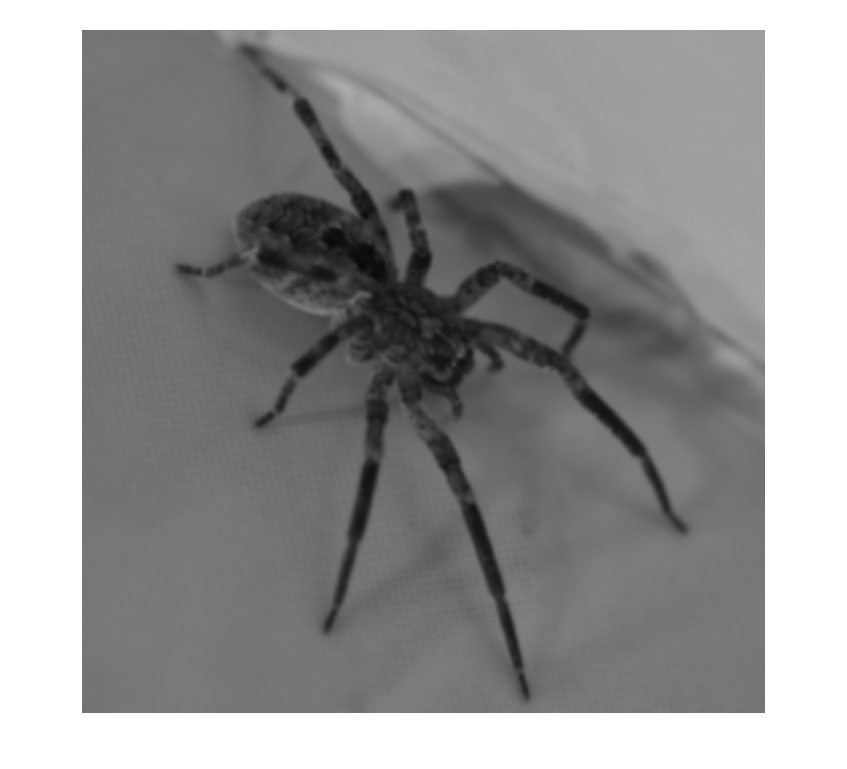
\includegraphics[width=\textwidth]{./figs/thresholding_sem_ruido.png}
                \caption{Imagem sem ruido}
                \label{fig:fundteor_sem_ruido}
		\fonte{\cite{MATHWORKS-HELP}}
        \end{subfigure}
       ~ %add desired spacing between images, e. g. ~, \quad, \qquad etc.
          %(or a blank line to force the subfigure onto a new line)
        \begin{subfigure}[b]{0.4\textwidth}
                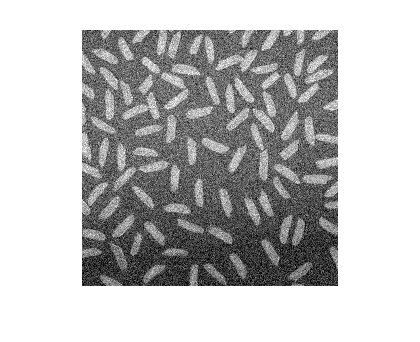
\includegraphics[width=\textwidth]{./figs/thresholding_ruido.png}
                \caption{Imagem com ruido}
                \label{fig:fundteor_com_ruido}
		\fonte{Autoria pr�pria}
        \end{subfigure}
        %add desired spacing between images, e. g. ~, \quad, \qquad etc.
        %(or a blank line to force the subfigure onto a new line)
        
	\begin{subfigure}[b]{0.4\textwidth}
                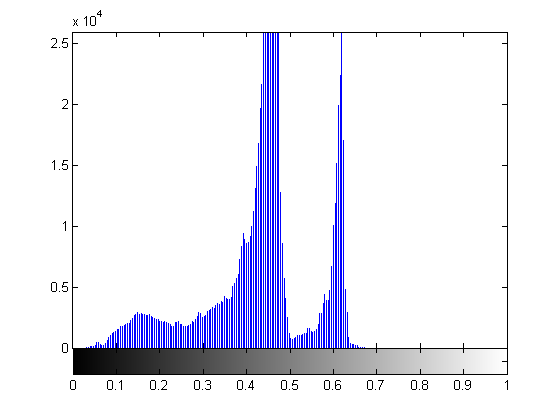
\includegraphics[width=\textwidth]{./figs/thresholding_histograma_sem_ruido.png}
                \caption{Histograma da imagem sem ruido}
                \label{fig:fundteor_hist_sem_ruido}
		\fonte{Autoria pr�pria}
        \end{subfigure}
       ~ %add desired spacing between images, e. g. ~, \quad, \qquad etc.
          %(or a blank line to force the subfigure onto a new line)
        \begin{subfigure}[b]{0.4\textwidth}
                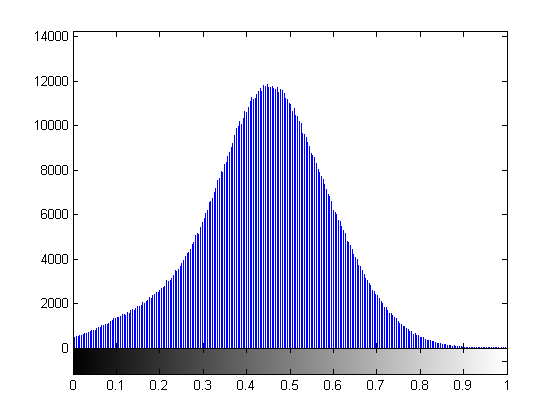
\includegraphics[width=\textwidth]{./figs/thresholding_histograma_ruido.png}
                \caption{Histograma da imagem com ruido}
                \label{fig:fundteor_hist_com_ruido}
		\fonte{Autoria pr�pria}
        \end{subfigure}
        %add desired spacing between images, e. g. ~, \quad, \qquad etc.
        %(or a blank line to force the subfigure onto a new line)

        \caption{Imagens com e sem ru�do e seus respectivos histogramas}
	\label{fig:fundteor_fig_limiarizacao}
\end{figure}

%\subsubsection{Limiariza��o global}
	% basic global thresholding

\subsubsection{Limiariza��o global pelo m�todo de \emph{Otsu}}
	% metodo de otsu
O m�todo para determinar o valor do limiar $T$ proposto por \emph{Otsu} � um m�todo �timo que busca maximizar a vari�ncia entre as duas classes. Isso baseia-se no fato de que classes bem divididas possuem valores de intensidades distintos, e o valor �timo para $T$ � o valor tal que haja maior separa��o entre as intensidades \cite{GONZALEZ-2006}.

O c�lculo do valor limiar pelo m�todo de \emph{Otsu} se d� pela equa��o \ref{eq:fundteor_otsu}.

\begin{equation}
\sigma _{B}^{2} (t) = \frac{\left [m_{G}P_{1}(t) - m(t)  \right ]^{2}}{P_{1}(t)\left [ 1 - P_{1}(t) \right ]}
\label{eq:fundteor_otsu}
\end{equation}

Onde:

\begin{itemize}
\item $\sigma _{B}^{2} (t)$ � a vari�ncia entre as classes para um valor limiar t;
\item $m_{G}$ � a m�dia global de intensidades da imagem;
\item $P_{1}(t)$ � a probabilidade de um pixel qualquer da imagem estar na classe 1 dado o valor limiar $t$.
\item $ m(t)$ � a m�dia acumulada das intensidades de $t=0$ at� a intensidade $t$;
\end{itemize}

Portanto, para o c�lculo do valor limiar pelo m�todo de \emph{Otsu} basta encontrar o valor limiar $t$ tal que q vari�ncia entre as classes, $\sigma _{B}^{2} (t)$, � m�ximo. A dedu��o da equa��o \ref{eq:fundteor_otsu} est� fora do escopo deste projeto, mas pode ser encontrada em \cite{GONZALEZ-2006}. 

Na figura \ref{fig:fundteor_fig_limiarizada} mostram-se as imagens da figura \ref{fig:fundteor_fig_limiarizacao} limiarizadas pelo m�todo de \emph{Otsu} e seus respectivos valores de limiariza��o.

\begin{figure}[H]
        \centering
	\begin{subfigure}[b]{0.4\textwidth}
                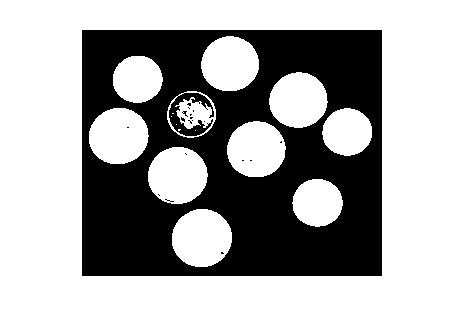
\includegraphics[width=\textwidth]{./figs/thresholded_sem_ruido.png}
                \caption{Imagem sem ruido limiarizada}
                \label{fig:fundteor_t_sem_ruido}
        \end{subfigure}
       ~ %add desired spacing between images, e. g. ~, \quad, \qquad etc.
          %(or a blank line to force the subfigure onto a new line)
        \begin{subfigure}[b]{0.4\textwidth}
                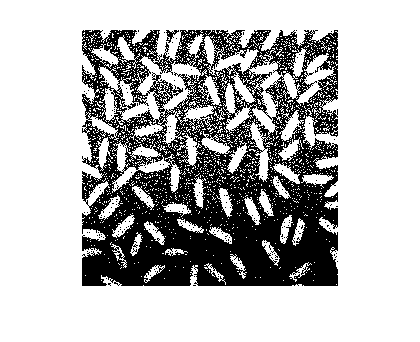
\includegraphics[width=\textwidth]{./figs/thresholded_ruido.png}
                \caption{Imagem com ruido limiarizada}
                \label{fig:fundteor_t_com_ruido}
        \end{subfigure}
        %add desired spacing between images, e. g. ~, \quad, \qquad etc.
        %(or a blank line to force the subfigure onto a new line)
        
	\begin{subfigure}[b]{0.4\textwidth}
                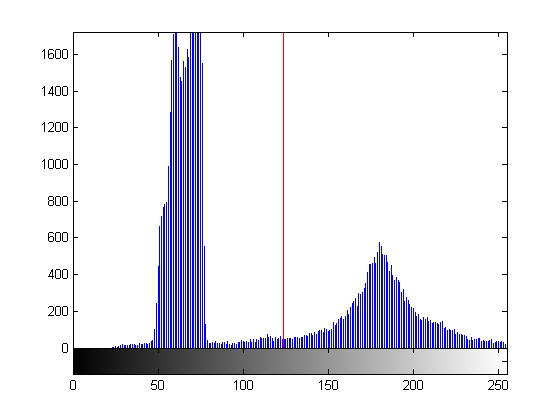
\includegraphics[width=\textwidth]{./figs/thresholded_histograma_sem_ruido.png}
                \caption{Histograma da imagem sem ruido com o valor do limiar T}
                \label{fig:fundteor_t_hist_sem_ruido}
        \end{subfigure}
       ~ %add desired spacing between images, e. g. ~, \quad, \qquad etc.
          %(or a blank line to force the subfigure onto a new line)
        \begin{subfigure}[b]{0.4\textwidth}
                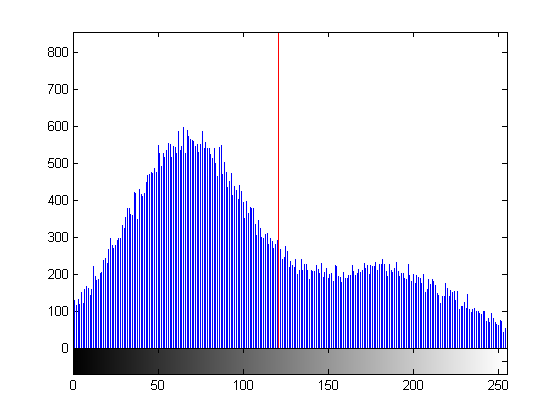
\includegraphics[width=\textwidth]{./figs/thresholded_histograma_ruido.png}
                \caption{Histograma da imagem com ruido com o valor do limiar T}
                \label{fig:fundteor_t_hist_com_ruido}
        \end{subfigure}
        %add desired spacing between images, e. g. ~, \quad, \qquad etc.
        %(or a blank line to force the subfigure onto a new line)

        \caption{Imagens limiarizadas pelo m�todo de \emph{Otsu} e seus respectivos histogramas}
	\fonte{Autoria pr�pria}
	\label{fig:fundteor_fig_limiarizada}
\end{figure}


\subsection{Opera��es morfol�gicas b�sicas} \label{sub:fundteor_op_morfologicas}

Opera��es morfol�gicas como abertura e fechamento podem ser �teis para filtrar imagens. Principalmente para filtrar imagens bin�rias onde a opera��o de fechamento pode ser aplicada para diminuir ruido.

Para o estudo das opera��es morfol�gicas de abertura e fechamento precisa-se primeiramente esclarecer alguns pontos:

\begin{itemize}
\item Podemos representar imagens bin�rias como sendo um conjunto de pixeis no espa�o $Z^2$, onde cada pixel � representado por uma tupla $(x,y)$ e $x$ e $y$ s�o as coordenadas do pixel.
\item A transla��o de um conjunto $B$ para um ponto $z = (z_{1},z_{2})$, denotado por $(B)_z$ � o conjunto de pontos em $B$ com as respectivas coordenas $(x,y)$ tendo sido substitu�das pela coordenadas $(x+z_{1}, y+z_{2})$.
\item Elemento estruturante � um conjunto de pixeis que � utilizado para fazer opera��es sobre uma imagem. Cada elemento estruturante possui um pixel de origem. A figura \ref{fig:fundteor_elementos_estruturantes} mostra exemplos de elementos estruturantes e suas respectivas origens.

\begin{figure}[H]
	\centering
	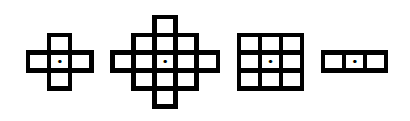
\includegraphics[width=0.8\textwidth]{./figs/elementos_estruturantes.png}
	\caption{Exemplos de elementos estruturantes.}
	\fonte{Autoria pr�pria}
	\label{fig:fundteor_elementos_estruturantes}
\end{figure}

\item O elemento estruturante pode ser utilizado para fazer opera��es sobre uma imagem bin�ria. Considere por exemplo a opera��o no conjunto $A$, feita pelo elemento estruturante $B$ (figuras \ref{fig:fundteor_elementos_estruturantes_ex_A} e \ref{fig:fundteor_elementos_estruturantes_ex_B}): Cria-se um novo conjunto $C$ sobrepondo $B$ em $A$ da maneira que a origem de $B$ passe por todos os pixeis de $A$. Em cada ponto que a origem de $B$ passa verifica-se se $B$ est� completamente contido em $A$. Se estiver marca-se esse ponto no conjunto $C$. A figura \ref{fig:fundteor_elementos_estruturantes_ex_C} mostra o resultado da opera��o, ou seja, o conjunto $C$.

\begin{figure}[H]
        \centering
	\begin{subfigure}[b]{0.4\textwidth}
                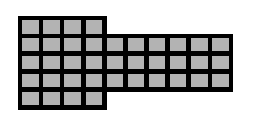
\includegraphics[width=\textwidth]{./figs/elementos_estruturantes_A.png}
                \caption{Imagem bin�ria $A$}
                \label{fig:fundteor_elementos_estruturantes_ex_A}
        \end{subfigure}
       ~ %add desired spacing between images, e. g. ~, \quad, \qquad etc.
          %(or a blank line to force the subfigure onto a new line)
        \begin{subfigure}[b]{0.4\textwidth}
                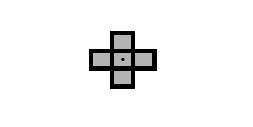
\includegraphics[width=\textwidth]{./figs/elementos_estruturantes_B.png}
                \caption{Elemento estruturante $B$}
                \label{fig:fundteor_elementos_estruturantes_ex_B}
        \end{subfigure}
        %add desired spacing between images, e. g. ~, \quad, \qquad etc.
        %(or a blank line to force the subfigure onto a new line)
        
	\begin{subfigure}[b]{0.4\textwidth}
                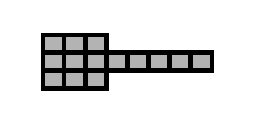
\includegraphics[width=\textwidth]{./figs/elementos_estruturantes_C.png}
                \caption{$C$, resultado da opera��o de $B$ em $A$}
                \label{fig:fundteor_elementos_estruturantes_ex_C}
        \end{subfigure}

        \caption{Imagem bin�ria, elemento estruturante e opera��o de $B$ em $A$}
	\fonte{Autoria pr�pria}
	\label{fig:elementos_estruturantes_ex}
\end{figure}

\end{itemize}

A seguir apresentam-se as opera��es de eros�o e de dilata��o, que s�o necess�rias para as opera��es de abertura e fechamento que s�o apresentadas na sequencia.


\subsubsection{Eros�o}

Sendo $A$ e $B$ conjuntos no espa�o $Z^2$, a eros�o do conjunto $A$ pelo elemento estruturante $B$, denotada por $A \ominus B$, � definida na equa��o \ref{eq:fundteor_erosao} \cite{GONZALEZ-2006}.

\begin{equation}
A \ominus B = \left \{ z \mid (B)_z \subseteq A) \right \}
\label{eq:fundteor_erosao}
\end{equation}

Ou seja, a eros�o de $A$ por $B$ � o conjunto de todos os pontos $z$ tal que $B$, transladado por $z$, est� completamente contido em $A$. Pode-se ver melhor esse processo na figura \ref{fig:fundteor_erosao_A_B}, onde o conjunto A � erodido pelo elemento estruturante B formando o conjunto $A \ominus B$.

\begin{figure}[H]
	\centering
	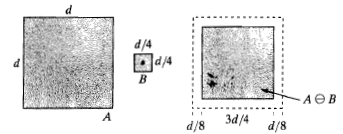
\includegraphics[width=0.8\textwidth]{./figs/erosao_A_B.png}
	\caption{Exemplo de eros�o do conjunto A por B.}
	\fonte{\cite{GONZALEZ-2006}}
	\label{fig:fundteor_erosao_A_B}
\end{figure}
 

\subsubsection{Dilata��o}

Sendo $A$ e $B$ conjuntos no espa�o $Z^2$, a dilata��o do conjunto $A$ pelo elemento estruturante $B$, denotada por $A \oplus  B$, � definida na equa��o \ref{eq:fundteor_dilatacao} \cite{GONZALEZ-2006}.

\begin{equation}
A \oplus B = \left \{ z\mid \left [(\hat{B})_{z} \cap A  \right ] \subseteq A \right \}
\label{eq:fundteor_dilatacao}
\end{equation}

Onde $\hat{B}$ � o conjunto $B$ espelhado. Quando o elemento estruturante � sim�trico ent�o $\hat{B}=B$. 

A equa��o \ref{eq:fundteor_dilatacao} diz que a dilata��o do conjunto $A$ pelo elemento estruturante $B$ � o conjunto de todos os pontos $z$ tal que se $\hat{B}$ e $A$ se sobrep�em em pelo menos um ponto, ent�o $z$ faz parte de $A \oplus B$. Pode-se ver melhor esse processo na figura \ref{fig:fundteor_dilatacao_A_B}, onde o conjunto $A$ � dilatado pelo elemento estruturante $B$ formando o conjunto $A \oplus B$.

\begin{figure}[H]
	\centering
	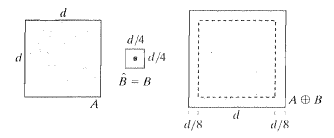
\includegraphics[width=0.8\textwidth]{./figs/dilatacao_A_B.png}
	\caption{Exemplo de dilata��o do conjunto A por B.}
	\fonte{\cite{GONZALEZ-2006}}
	\label{fig:fundteor_dilatacao_A_B}
\end{figure}


\subsubsection{Abertura e Fechamento}

A abertura do conjunto $A$ pelo elemento estruturante $B$ � definida pela equa��o \ref{eq:fundteor_abertura}  \cite{GONZALEZ-2006}.

\begin{equation}
A \circ B = \left ( A \ominus B \right ) \oplus B
\label{eq:fundteor_abertura}
\end{equation}

O fechamento do conjunto $A$ pelo elemento estruturante $B$ � definido pela equa��o \ref{eq:fundteor_fechamento}  \cite{GONZALEZ-2006}.

\begin{equation}
A \bullet B = \left ( A \oplus B \right ) \ominus B
\label{eq:fundteor_fechamento}
\end{equation}

Na figura \ref{fig:regiao_abertura} pode-se ver o resultado da execu��o da opera��o de abertura em cima do conjunto $A$ da figura \ref{fig:regiao_teste_A}. Em seguida na figura \ref{fig:regiao_fechamento} pode-se ver o resultado da execu��o da opera��o de fechamento em cima do mesmo conjunto da figura \ref{fig:regiao_teste_A}. Como pode-se ver, a opera��o de abertura "abre" a imagem em pontos estreitos, j� a opera��o de fechamento "fecha" a imagem onde existem cavidades pequenas.

\begin{figure}[H]
	\centering
	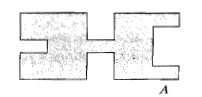
\includegraphics[width=0.5\textwidth]{./figs/regiao_teste.png}
	\caption{Conjunto $A$.}
	\fonte{\cite{GONZALEZ-2006}}
	\label{fig:regiao_teste_A}
\end{figure}

\begin{figure}[H]
	\centering
	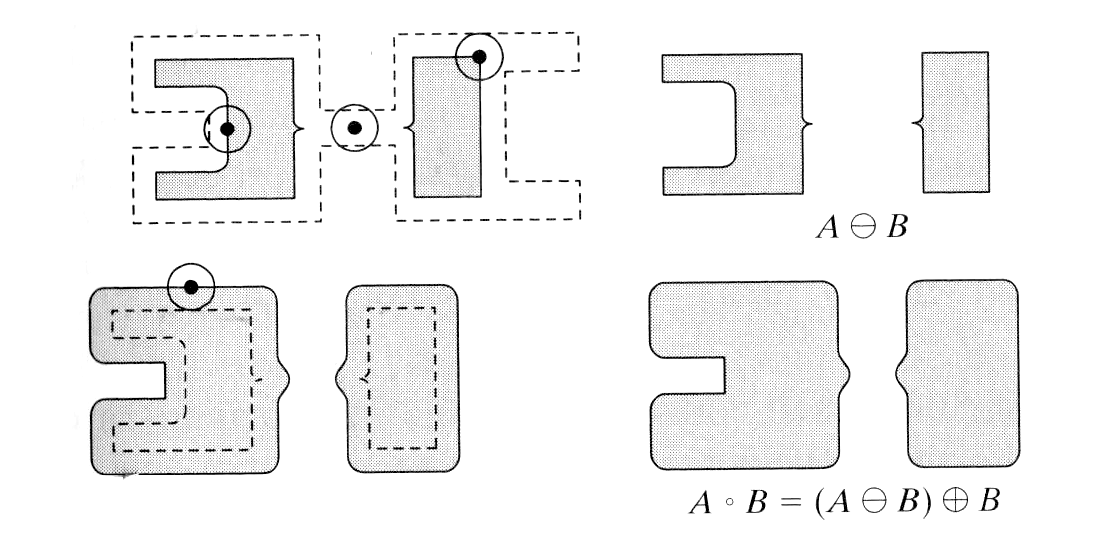
\includegraphics[width=0.8\textwidth]{./figs/regiao_abertura.png}
	\caption{Conjunto $A \circ B$.}
	\fonte{\cite{GONZALEZ-2006}}
	\label{fig:regiao_abertura}
\end{figure}

\begin{figure}[H]
	\centering
	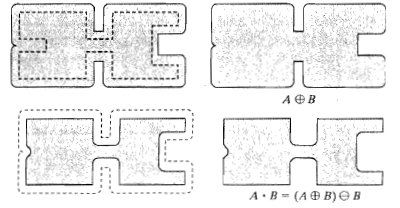
\includegraphics[width=0.8\textwidth]{./figs/regiao_fechamento.png}
	\caption{Conjunto $A \bullet B$.}
	\fonte{\cite{GONZALEZ-2006}}
	\label{fig:regiao_fechamento}
\end{figure}


\subsection{Esqueletoniza��o}

Define-se esqueleto conforme segue \cite{GONZALEZ-2006}.

Se $S(A)$ � o esqueleto de $A$ e $(D)_{z}$ o maior disco centrado em $z$ e contido em $A$, pode se dizer que :

\begin{itemize}
\item Se $z$ faz parte de $S(A)$ ent�o n�o � poss�vel encontrar um disco maior que $(D)_{z}$, n�o necessariamente centrado em $z$, que contenha $(D)_{z}$ e que esteja completamente incluso em $A$;
\item O disco $(D)_{z}$ toca a borda de $A$ em pelo menos dois pontos distintos.
\end{itemize}

Isso pode ser visto melhor na figura \ref{fig:esqueletonizacao_exemplo}.

\begin{figure}[H]
	\centering
	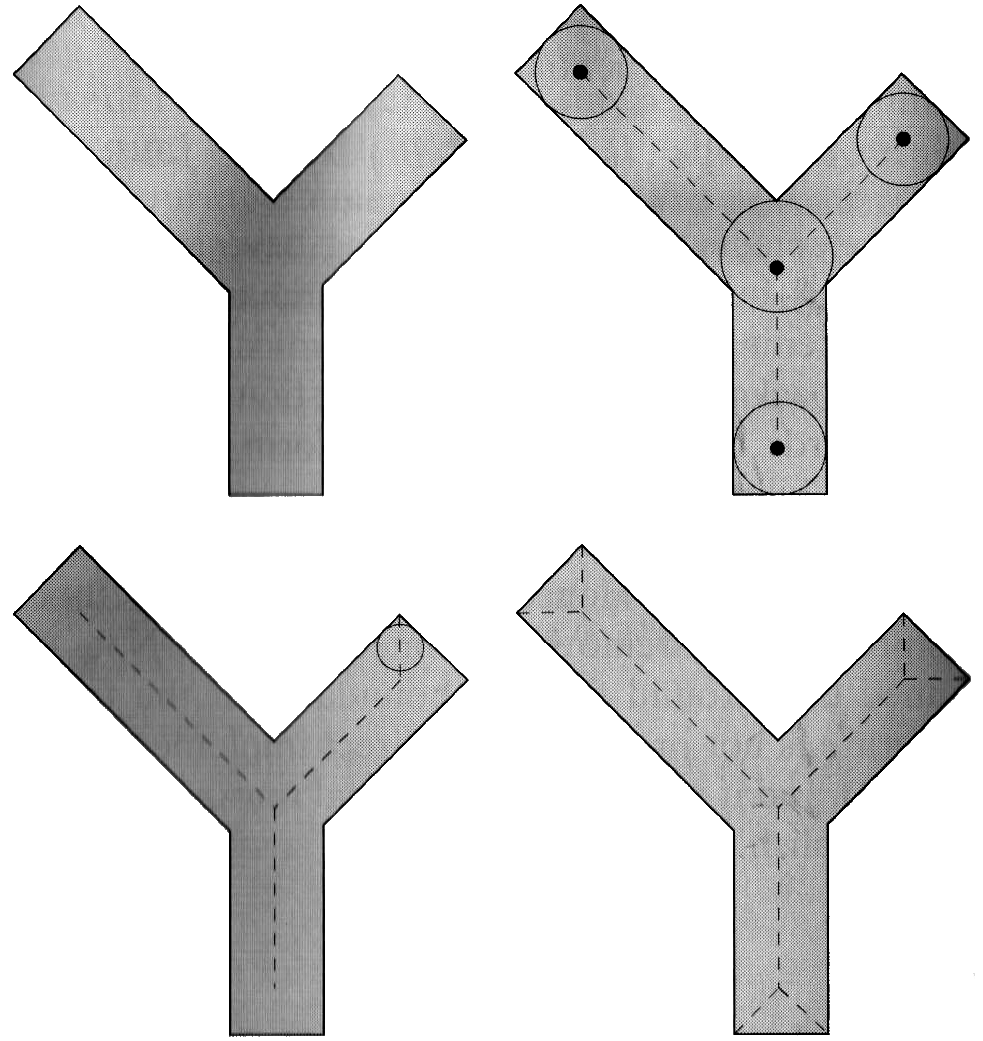
\includegraphics[width=0.8\textwidth]{./figs/esqueletonizacao_exemplo.png}
	\caption{Conjunto $A$, disco m�ximo centrado em diversos pontos $z$ e esqueleto completo.}
	\fonte{\cite{GONZALEZ-2006}}
	\label{fig:esqueletonizacao_exemplo}
\end{figure}

Pode-se definir tamb�m o esqueleto $S(A)$ em fun��o de eros�es e aberturas sucessivas como mostrado nas equa��es \ref{eq:fundteor_esqueletonizacao_1}, \ref{eq:fundteor_esqueletonizacao_2}, \ref{eq:fundteor_esqueletonizacao_3} e \ref{eq:fundteor_esqueletonizacao_4} \cite{GONZALEZ-2006}.

\begin{equation}
S(A) = \bigcup_{k = 0}^{K} S_{k}(A)
\label{eq:fundteor_esqueletonizacao_1}
\end{equation}

Com:

\begin{equation}
S_{k}(A) = (A \ominus k B) - (A \ominus k B) \circ B
\label{eq:fundteor_esqueletonizacao_2}
\end{equation}

Onde $B$ � um elemento estruturante e $(A \ominus k B)$ indica $k$ sucessivas eros�es de $A$:

\begin{equation}
(A \ominus k B) = ((...((A \ominus B) \ominus B) \ominus ...) \ominus B)
\label{eq:fundteor_esqueletonizacao_3}
\end{equation}

Sendo K o ultimo passo antes de $A$ erodir para um conjunto vazio. Ou seja:

\begin{equation}
K = max \left \{ k \mid (A \ominus k B) \neq \varnothing  \right \}
\label{eq:fundteor_esqueletonizacao_4}
\end{equation}


\subsubsection {Poda (\emph{Pruning})}

Aplicando-se o m�todo de esqueletoniza��o mencionado anteriormente em figuras reais, como a figura \ref{fig:fundteor_sketon_in}, pode-se obter resultados como a figura \ref{fig:fundteor_sketon_out}. Devido a esse tipo de resultados aplica-se ap�s a esqueletoniza��o um m�todo de poda. A poda do esqueleto consiste em avaliar o tamanho dos ramos gerados, caso sejam menores que um valor limiar s�o removidos. A figura \ref{fig:fundteor_sketon_out_20} mostra o m�todo de poda aplicado com um limiar de 20 pixeis.

\begin{figure}[H]
        \centering
	\begin{subfigure}[b]{0.49\textwidth}
                
\includegraphics[width=\textwidth]{./figs/skeleton_in.png}
                \caption{Imagem de entrada}
                \label{fig:fundteor_sketon_in}
        \end{subfigure}

       ~ %add desired spacing between images, e. g. ~, \quad, \qquad etc.
          %(or a blank line to force the subfigure onto a new line)
        \begin{subfigure}[b]{0.49\textwidth}
               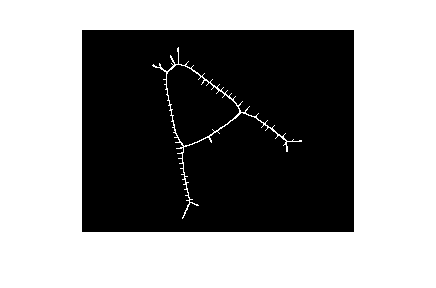
\includegraphics[width=\textwidth]{./figs/skeleton_out.png}
                \caption{Imagem esqueletonizada}
                \label{fig:fundteor_sketon_out}
        \end{subfigure}
        %add desired spacing between images, e. g. ~, \quad, \qquad etc.
        %(or a blank line to force the subfigure onto a new line)
	\begin{subfigure}[b]{0.49\textwidth}
                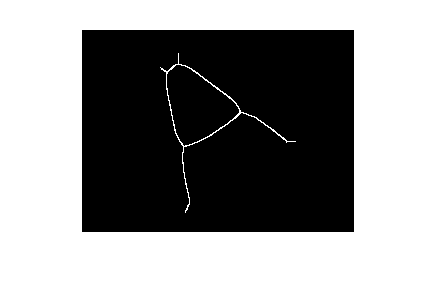
\includegraphics[width=\textwidth]{./figs/skeleton_out_20.png}
                \caption{Imagem esqueletonizada e podada}
                \label{fig:fundteor_sketon_out_20}
        \end{subfigure}

        \caption{Exemplo de esqueletoniza��o e poda.}
	\fonte{Autoria pr�pria}
	\label{fig:fundteor_sketon}
\end{figure}


\subsection{Normaliza��o}

A an�lise de componentes principais pode ser empregada para normalizar imagens em fun��o de rota��o, transla��o e tamanho  \cite{GONZALEZ-2006}. Explica-se a seguir alguns conceitos necess�rios para efetuar a normaliza��o utilizando a analise de componentes principais e em seguida o processo de normaliza��o utilizando componentes principais.

\subsubsection{Matriz de covari�ncias}

Considere as imagens da figura \ref{fig:fundteor_pca}. Os pontos da imagem, podem ser considerados como sendo vetores $x_{k}=(x_{1},x_{2})^{T}$, onde $x_{1}$ e $x_{2}$ s�o as coordenadas do ponto $x_{k}$, e $T$ indica a matriz transposta. Os pontos $x$ portanto formam uma popula��o de vetores no espa�o $Z^{2}$. Sendo assim pode-se calcular a matriz de covari�ncias $C_{x}$ e o vetor da m�dia $m_{x}$ para a popula��o de vetores.

Para $K$ amostras de uma popula��o aleat�ria pode-se aproximar a m�dia $m_{x}$ pela equa��o \ref{eq:fundteor_mean} \cite{GONZALEZ-2006}.

\begin{equation}
m_{x} = \frac{1}{K} \sum_{k=1}^{K} x_{k}
\label{eq:fundteor_mean}
\end{equation}

Agora utilizando a m�dia $m_{x}$, pode-se aproximar a matriz de covari�ncias $C_{x}$ pela equa��o \ref{eq:fundteor_cov} \cite{GONZALEZ-2006}.

\begin{equation}
C_{x} = \frac{1}{K} \sum_{k=1}^{K} (x_{k} x_{k}^{T}) - m_{x}m_{x}^{T}
\label{eq:fundteor_cov}
\end{equation}

Na matriz de covari�ncias os elementos $c_{ii}$ de $C_{x}$ representam a vari�ncia entre os valores na coordenada $x_{i}$. Os elementos $c_{ij}$ representam a covari�ncia entre os valores na coordenada $x_{i}$ com os valores da coordenada $x_{j}$. Portanto, a matriz de covari�ncia possui informa��es que dizem respeito � distribui��o dos pixeis da imagem. 

Pode-se ver isso melhor nas matrizes de covari�ncia apresentadas nas figuras \ref{fig:fundteor_pca_xc}, \ref{fig:fundteor_pca_yc} e \ref{fig:fundteor_pca_xyc} que foram calculadas para as imagens das figuras \ref{fig:fundteor_pca_x}, \ref{fig:fundteor_pca_y} e \ref{fig:fundteor_pca_xy} respectivamente. Percebe-se que na figura \ref{fig:fundteor_pca_xc} a maior vari�ncia ocorre entre os elementos da coordenada $x_{1}$, visto que $c_{11}$ possui o maior valor na matriz de covari�ncias. Semelhantemente percebe-se que na figura \ref{fig:fundteor_pca_yc} a maior vari�ncia ocorre entre os elementos da coordenada $x_2$. A terceira imagem, figura \ref{fig:fundteor_pca_xyc}, mostra uma distribui��o mais continua em $x_{1}$ e $x_{2}$, mas valores maiores para as covari�ncias entre os elementos das coordenadas $x_{1}$ e $x_{2}$. A terceira imagem mostra portanto o relacionamento entre as duas coordenadas da imagem: quando  $x_{1}$ aumenta,  $x_{2}$ tende a aumentar tamb�m, e vice-versa.

\begin{figure}[H]
        \centering
	\begin{subfigure}[b]{0.3\textwidth}
                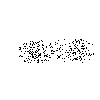
\includegraphics[width=\textwidth]{./figs/pca_x.png}
	        \caption{}
                \label{fig:fundteor_pca_x}
        \end{subfigure}
       ~ %add desired spacing between images, e. g. ~, \quad, \qquad etc.
          %(or a blank line to force the subfigure onto a new line)
        \begin{subfigure}[b]{0.3\textwidth}
                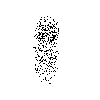
\includegraphics[width=\textwidth]{./figs/pca_y.png}
	        \caption{}
                \label{fig:fundteor_pca_y}
        \end{subfigure}
       ~ %add desired spacing between images, e. g. ~, \quad, \qquad etc.
          %(or a blank line to force the subfigure onto a new line)
	\begin{subfigure}[b]{0.3\textwidth}
                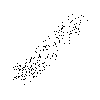
\includegraphics[width=\textwidth]{./figs/pca_xy.png}
	        \caption{}
                \label{fig:fundteor_pca_xy}
        \end{subfigure}

	\begin{subfigure}[b]{0.3\textwidth}
		\centerline{$\begin{bmatrix}
			457 & -13.6 \\ 
			-13.6 & 35.0
		\end{bmatrix}$}
	        \caption{}
                \label{fig:fundteor_pca_xc}
        \end{subfigure}
       ~ %add desired spacing between images, e. g. ~, \quad, \qquad etc.
          %(or a blank line to force the subfigure onto a new line)
        \begin{subfigure}[b]{0.3\textwidth}
		\centerline{$\begin{bmatrix}
			39.1 & -8.30 \\ 
			-8.30 & 263
		\end{bmatrix}$}
	        \caption{}
                \label{fig:fundteor_pca_yc}
        \end{subfigure}
       ~ %add desired spacing between images, e. g. ~, \quad, \qquad etc.
          %(or a blank line to force the subfigure onto a new line)
	\begin{subfigure}[b]{0.3\textwidth}
		\centerline{$\begin{bmatrix}
			360 & -318 \\ 
			-318 & 343
		\end{bmatrix}$}
	        \caption{}
                \label{fig:fundteor_pca_xyc}
        \end{subfigure}

        \caption{Imagens de exemplo e suas respectivas matrizes de covari�ncia.}
	\fonte{Autoria pr�pria}
	\label{fig:fundteor_pca}
\end{figure}

\subsubsection{Autovetores e autovalores}

Um autovetor de uma matriz $A$ � um vetor n�o nulo $v$, que quando a matriz � multiplicada por $v$ tem-se um vetor que � m�ltiplo de $v$ por uma constante $\lambda$ denominada autovalor. Ou seja, a equa��o \ref{eq:fundteor_eigen} � verdadeira \cite{AUTOVETORES}.

\begin{equation}
Av = \lambda v
\label{eq:fundteor_eigen}
\end{equation}

Algumas propriedades de autovetores:

\begin{itemize}
\item Os autovetores podem ser calculados apenas para matrizes quadradas \cite{AUTOVETORES};
\item Para uma matriz $nxn$ existem $n$ autovetores \cite{AUTOVETORES};
\item Todos os autovetores s�o ortogonais entre si \cite{GONZALEZ-2006}.
\end{itemize}

\subsubsection{Analise de componentes principais}

% http://www.cs.otago.ac.nz/cosc453/student_tutorials/principal_components.pdf
% https://inst.eecs.berkeley.edu/~ee127a/book/login/l_sym_pca.html
Pode-se demonstrar que o autovetor associado ao maior autovalor de uma matriz de covari�ncias aponta na dire��o de maior varia��o dos dados \cite{AUTOVETORES-DEDUCAO}. Pode-se demonstrar tamb�m que o segundo autovetor, associado ao segundo maior autovalor, aponta na segunda dire��o de maior varia��o dos dados. A esses autovetores se d� o nome de componentes principais da imagem.

Considere por exemplo as imagens da figura \ref{fig:fundteor_pca2}. Calculamos os autovetores para cada uma das imagens tomando como base as matrizes de covari�ncia apresentadas nas figuras \ref{fig:fundteor_pca_xc}, \ref{fig:fundteor_pca_yc} e \ref{fig:fundteor_pca_xyc}. Os autovetores podem ser vistos nas figuras \ref{fig:fundteor_pca_xam}, \ref{fig:fundteor_pca_yam} e \ref{fig:fundteor_pca_xyam}. O autovetor associado ao maior autovalor est� na primeira linha de cada matriz e o segundo autovetor est� na segunda linha. Os autovetores foram representados sobre as respectivas imagens nas figuras \ref{fig:fundteor_pca_xa}, \ref{fig:fundteor_pca_ya} e \ref{fig:fundteor_pca_xya}.

\begin{figure}[H]
        \centering
	\begin{subfigure}[b]{0.3\textwidth}
                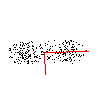
\includegraphics[width=\textwidth]{./figs/pca_xa.png}
	        \caption{}
                \label{fig:fundteor_pca_xa}
        \end{subfigure}
       ~ %add desired spacing between images, e. g. ~, \quad, \qquad etc.
          %(or a blank line to force the subfigure onto a new line)
        \begin{subfigure}[b]{0.3\textwidth}
                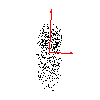
\includegraphics[width=\textwidth]{./figs/pca_ya.png}
	        \caption{}
                \label{fig:fundteor_pca_ya}
        \end{subfigure}
       ~ %add desired spacing between images, e. g. ~, \quad, \qquad etc.
          %(or a blank line to force the subfigure onto a new line)
	\begin{subfigure}[b]{0.3\textwidth}
                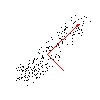
\includegraphics[width=\textwidth]{./figs/pca_xya.png}
	        \caption{}
                \label{fig:fundteor_pca_xya}
        \end{subfigure}

	\begin{subfigure}[b]{0.3\textwidth}
		\centerline{$\begin{bmatrix}
			0.999 & 0.0321 \\ 
			0.0321 & -0.999
		\end{bmatrix}$}
	        \caption{}
                \label{fig:fundteor_pca_xam}
        \end{subfigure}
       ~ %add desired spacing between images, e. g. ~, \quad, \qquad etc.
          %(or a blank line to force the subfigure onto a new line)
        \begin{subfigure}[b]{0.3\textwidth}
		\centerline{$\begin{bmatrix}
			0.0369 & 0.999 \\ 
			0.999 & -0.0369
		\end{bmatrix}$}
	        \caption{}
                \label{fig:fundteor_pca_yam}
        \end{subfigure}
       ~ %add desired spacing between images, e. g. ~, \quad, \qquad etc.
          %(or a blank line to force the subfigure onto a new line)
	\begin{subfigure}[b]{0.3\textwidth}
		\centerline{$\begin{bmatrix}
			0.716 & 0.698 \\ 
			0.698 & -0.716
		\end{bmatrix}$}
	        \caption{}
                \label{fig:fundteor_pca_xyam}
        \end{subfigure}

        \caption{Imagens de exemplo e seus respectivos autovetores.}
	\fonte{Autoria pr�pria}
	\label{fig:fundteor_pca2}
\end{figure}

V�-se portanto que � poss�vel definir um eixo absoluto para cada imagem com base na distribui��o dos pixeis sobre a imagem.

\subsubsection{Normaliza��o}

A normaliza��o das imagens pode ser feita por meio de uma matriz de transforma��o que mapeia valores do sistema de coordenadas original da imagem para o sistema de coordenadas formado pelos autovetores da imagem \cite{GONZALEZ-2006}. A transforma��o em quest�o podes ser expressa pela equa��o \ref{eq:fundteor_transf}.

\begin{equation}
y = A ( x - m_{x} )
\label{eq:fundteor_transf}
\end{equation}

Onde:

\begin{itemize}
\item $y$ � o valor no novo sistema de coordenadas formado pelos autovetores.
\item $x$ o valor da coordenada no sistema original.
\item $A$ a matriz de autovetores.
\item $m_{x}$ vetor da m�dia.
\end{itemize}

As imagens da figura \ref{fig:fundteor_pca} podem ser vistas normalizadas na figura \ref{fig:fundteor_pca3}.

\begin{figure}[H]
        \centering
	\begin{subfigure}[b]{0.3\textwidth}
                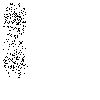
\includegraphics[width=\textwidth]{./figs/pca_xn.png}
	        \caption{}
                \label{fig:fundteor_pca_xa}
        \end{subfigure}
       ~ %add desired spacing between images, e. g. ~, \quad, \qquad etc.
          %(or a blank line to force the subfigure onto a new line)
        \begin{subfigure}[b]{0.3\textwidth}
                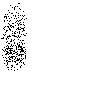
\includegraphics[width=\textwidth]{./figs/pca_yn.png}
	        \caption{}
                \label{fig:fundteor_pca_ya}
        \end{subfigure}
       ~ %add desired spacing between images, e. g. ~, \quad, \qquad etc.
          %(or a blank line to force the subfigure onto a new line)
	\begin{subfigure}[b]{0.3\textwidth}
                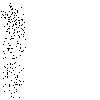
\includegraphics[width=\textwidth]{./figs/pca_xyn.png}
	        \caption{}
                \label{fig:fundteor_pca_xya}
        \end{subfigure}

        \caption{Imagens normalizadas.}
	\fonte{Autoria pr�pria}
	\label{fig:fundteor_pca3}
\end{figure}

Caso se deseje normalizar a imagem com rela��o ao tamanho pode-se dividir o valor das coordenadas $y$ pelos autovalores correspondentes \cite{GONZALEZ-2006}.


\section{Descri��o} \label{sec:descricao}

Esta se��o apresenta t�cnicas e algoritmos para realizar a descri��o de imagens, tais como extra��o de propriedades b�sicas de regi�es e descritores de \emph{fourier}.


\subsection{Propriedades de regi�es}

Propriedades b�sicas de regi�es, como �rea e excentricidade, podem ser usadas para descrever imagens. A seguir descreve-se algumas propriedades b�sicas de regi�es, principalmente aquelas que possuem como sa�da um valor escalar, visto que s�o facilmente adicionados � um vetor descritor.

\subsubsection{�rea}

A �rea de uma regi�o � o n�mero de pixeis da regi�o \cite{MATHWORKS-HELP-2}.

\subsubsection{�rea convexa}

A �rea convexa � dada pela �rea do menor pol�gono capaz de conter a regi�o \cite{MATHWORKS-HELP-2}.

\subsubsection{�rea Preenchida}

�rea preenchida corresponde a �rea da regi�o cujas cavidades foram todas preenchidas \cite{MATHWORKS-HELP-2}.

\subsubsection{Solidez}

A solidez de uma regi�o � dada pela raz�o �rea / �rea convexa \cite{MATHWORKS-HELP-2}.

\subsubsection{Extens�o}

Semelhantemente � �rea convexa, a extens�o � dada pela raz�o entre a �rea da regi�o (definida anteriormente) e a �rea do menor ret�ngulo capaz de conter a regi�o \cite{MATHWORKS-HELP-2}.

\subsubsection{Excentricidade}

Para a obten��o da excentricidade de uma regi�o deve-se primeiramente obter o momento de in�rcia de �rea da regi�o \cite{MATHWORKS-HELP-2}. O momento de in�rcia de �rea para uma regi�o qualquer no sistema de coordenadas polares � definido pela equa��o \ref{eq:fundteor_mom_in}:

\begin{equation}
J_{BB} = \int_{A}^{ } \rho ^{2} dA
\label{eq:fundteor_mom_in}
\end{equation}

Onde $A$ � a �rea da regi�o sobre a qual se deseja calcular o momento de in�rcia de �rea e $\rho$ � a dist�ncia do centro do sistema de coordenadas at� $dA$. Uma representa��o da �rea pode ser vista na figura \ref{fig:fundteor_mom_in_fig}.

\begin{figure}[H]
	\centering
	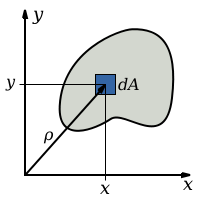
\includegraphics[width=0.3\textwidth]{./figs/Polar_Moment_of_Inertia.png}
	\caption{Representa��o da �rea para c�lculo do momento de in�rcia.}
	\fonte{\cite{IMAGEM-MOMENTO-INERCIA}}
	\label{fig:fundteor_mom_in_fig}
\end{figure}

A excentricidade da regi�o � ent�o a excentricidade da elipse que possui o mesmo momento de in�rcia que a �rea da regi�o.
A excentricidade para uma elipse com semi-eixo maior $a$ e semi-eixo menor $b$ � dada pela equa��o \ref{eq:fundteor_exc}:

\begin{equation}
e = \sqrt{1 - \frac{b^2}{a^2}}
\label{eq:fundteor_exc}
\end{equation}

\subsubsection{Tamanho do eixo principal e eixo secund�rio}

O tamanho do eixo principal de uma regi�o diz respeito ao tamanho do maior eixo da elipse que possui o mesmo momento de in�rcia de �rea que a �rea da regi�o, conforme visto anteriormente na se��o Excentricidade \cite{MATHWORKS-HELP-2}. Da mesma forma o tamanho do eixo secund�rio diz respeito ao tamanho do menor eixo da elipse que possui o mesmo momento de in�rcia de �rea que a �rea da regi�o.

\subsubsection{N�mero de Euler}

O n�mero de Euler � dado pelo total de objetos desconexos da regi�o subtraindo o total de cavidades da regi�o \cite{MATHWORKS-HELP-2}.


\subsection{Descritores de \emph{fourier}}

Considere a figura \ref{fig:fundteor_fourier_desc_org}. Os pixeis com valor $1$ da imagem bin�ria podem ser representados como sendo pares de coordenadas $(x_{0},y_{0}),(x_{1},y_{1}),(x_{2},y_{2}),...,(x_{K-1},y_{K-1})$, onde $K$ � o n�mero de pixeis na imagem. Al�m disso os pixeis podem ser representados como uma sequencia $x(k) = x_{k}$ e $y(k) = y_{k}$ ou como $s(k) = \left [ x(k), y(k) \right ]$ para $k = 0,1,2,...,K-1$. Al�m disso pode-se tratar as coordenadas dos pixeis como n�meros complexos: $s(k) = x(k) + j y(k)$.

Tem-se que a transformada discreta de \emph{fourier} de um sinal $s(k)$ � dado pela equa��o \ref{eq:fundteor_dft} \cite{GONZALEZ-2006}:

\begin{equation}
a(u) = \sum_{k=0}^{K-1} s(k) e^{-j2 \pi u k / K} ~~~~~ ,u = 0,1,2,...,K-1
\label{eq:fundteor_dft}
\end{equation}

Os coeficientes complexos $a(u)$ da transformada discreta de \emph{fourier} s�o chamados de descritores de \emph{fourier} \cite{GONZALEZ-2006}.

Da mesma forma que se aplicou a transformada discreta de \emph{fourier} para obter os descritores de \emph{fourier} pode-se aplicar a transformada discreta inversa de \emph{fourier} nos coeficientes complexos para obter novamente os n�meros complexos representando as coordenadas dos pixeis (equa��o \ref{eq:fundteor_idft}).

\begin{equation}
s(k) = \frac{1}{K} \sum_{u=0}^{K-1} a(u) e^{j2 \pi u k / K} ~~~~~ ,k = 0,1,2,...,K-1
\label{eq:fundteor_idft}
\end{equation}

Suponha agora que ao inv�s de utilizar todos os descritores de \emph{fourier} utiliza-se apenas os $P$ primeiros descritores para reconstituir $s(k)$. Tem-se portanto uma aproxima��o para $s(k)$ dada por $\hat{s}(k)$ na equa��o \ref{eq:fundteor_idft_a}.

\begin{equation}
\hat{s}(k) = \frac{1}{P} \sum_{u=0}^{P-1} a(u) e^{j2 \pi u k / P} ~~~~~ ,k = 0,1,2,...,K-1
\label{eq:fundteor_idft_a}
\end{equation}

Quando os $P$ coeficientes de menor frequ�ncia s�o escolhidos para reconstituir a imagem tem-se uma imagem aproximada da imagem original por�m que mant�m as principais caracter�sticas. Pode-se ver esse comportamento nas imagens da figura \ref{fig:fundteor_fourier_desc}. A imagem da figura \ref{fig:fundteor_fourier_desc_1} foi forma utilizando todos os 19410 coeficientes da imagem original, a imagem \ref{fig:fundteor_fourier_desc_2} foi formada com 9705 coeficientes, e assim por diante, at� apenas 2 coeficientes na figura \ref{fig:fundteor_fourier_desc_8192}.

\begin{figure}[H]
        \centering
	\begin{subfigure}[b]{0.29\textwidth}
                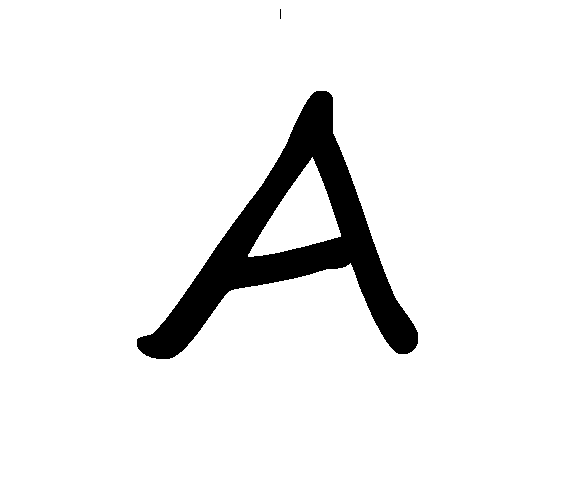
\includegraphics[width=\textwidth]{./figs/Ai.png}
	        \caption{Imagem original}
                \label{fig:fundteor_fourier_desc_org}
        \end{subfigure}
       ~ %add desired spacing between images, e. g. ~, \quad, \qquad etc.
          %(or a blank line to force the subfigure onto a new line)
	\begin{subfigure}[b]{0.29\textwidth}
                
\includegraphics[width=\textwidth]{./figs/A1.png}
	        \caption{19410 coeficientes}
                \label{fig:fundteor_fourier_desc_1}
        \end{subfigure}
	~ %add desired spacing between images, e. g. ~, \quad, \qquad etc.
          %(or a blank line to force the subfigure onto a new line)
	\begin{subfigure}[b]{0.29\textwidth}
                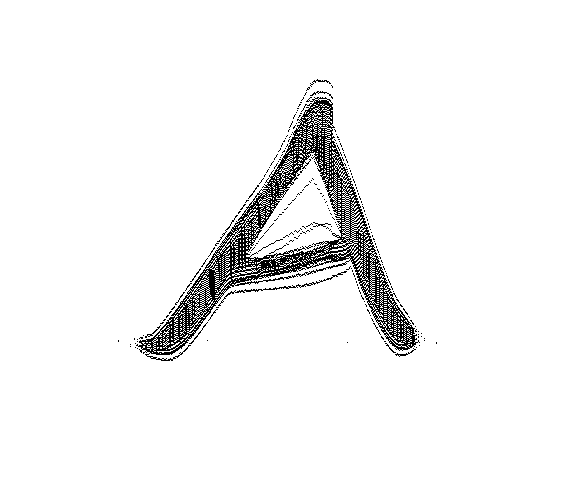
\includegraphics[width=\textwidth]{./figs/A2.png}
	        \caption{9705 coeficientes}
                \label{fig:fundteor_fourier_desc_2}
        \end{subfigure}

	\begin{subfigure}[b]{0.29\textwidth}
                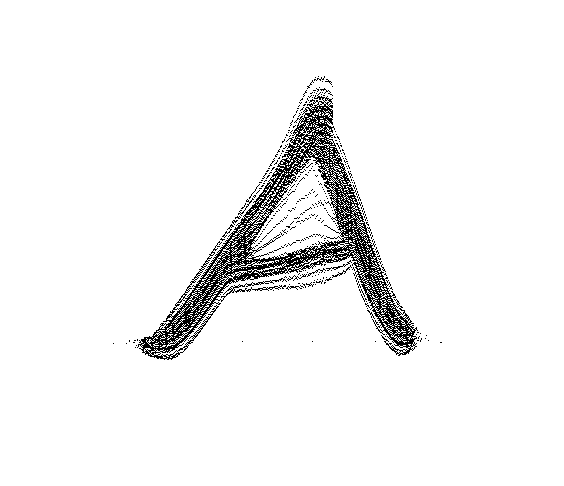
\includegraphics[width=\textwidth]{./figs/A4.png}
	        \caption{4852 coeficientes}
                \label{fig:fundteor_fourier_desc_4}
        \end{subfigure}
	~ %add desired spacing between images, e. g. ~, \quad, \qquad etc.
          %(or a blank line to force the subfigure onto a new line)
	\begin{subfigure}[b]{0.29\textwidth}
                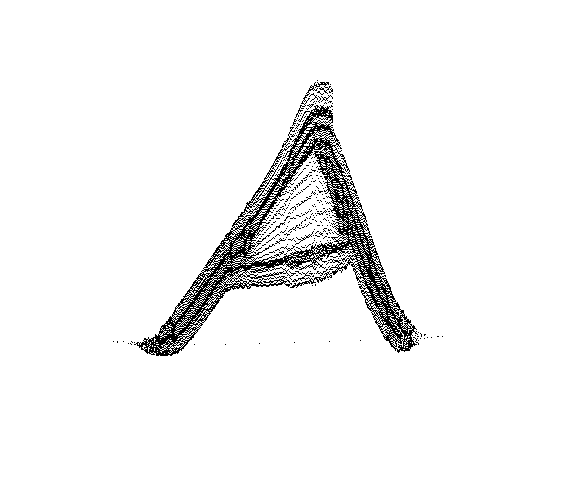
\includegraphics[width=\textwidth]{./figs/A8.png}
	        \caption{2426 coeficientes}
                \label{fig:fundteor_fourier_desc_8}
        \end{subfigure}
	~ %add desired spacing between images, e. g. ~, \quad, \qquad etc.
          %(or a blank line to force the subfigure onto a new line)
	\begin{subfigure}[b]{0.29\textwidth}
                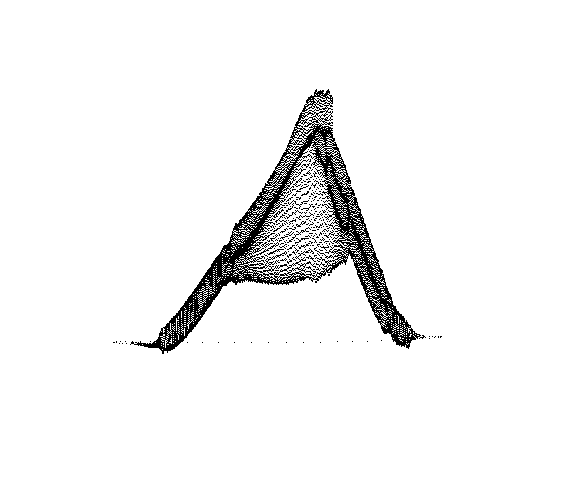
\includegraphics[width=\textwidth]{./figs/A16.png}
	        \caption{1213 coeficientes}
                \label{fig:fundteor_fourier_desc_16}
        \end{subfigure}

	\begin{subfigure}[b]{0.29\textwidth}
                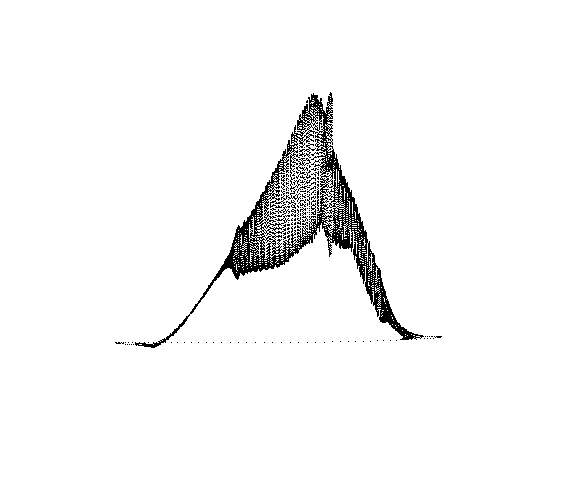
\includegraphics[width=\textwidth]{./figs/A32.png}
	        \caption{606 coeficientes}
                \label{fig:fundteor_fourier_desc_32}
        \end{subfigure}
	~ %add desired spacing between images, e. g. ~, \quad, \qquad etc.
          %(or a blank line to force the subfigure onto a new line)
	\begin{subfigure}[b]{0.29\textwidth}
                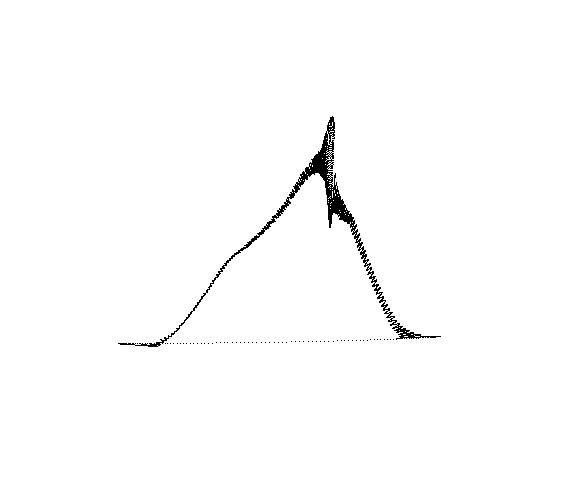
\includegraphics[width=\textwidth]{./figs/A64.png}
	        \caption{303 coeficientes}
                \label{fig:fundteor_fourier_desc_64}
        \end{subfigure}
	~ %add desired spacing between images, e. g. ~, \quad, \qquad etc.
          %(or a blank line to force the subfigure onto a new line)
	\begin{subfigure}[b]{0.29\textwidth}
                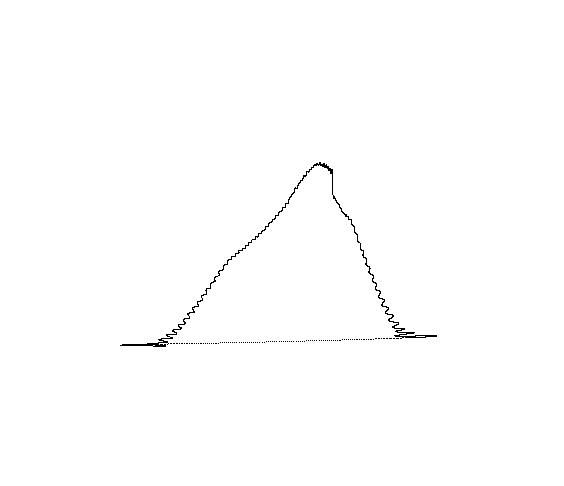
\includegraphics[width=\textwidth]{./figs/A128.png}
	        \caption{151 coeficientes}
                \label{fig:fundteor_fourier_desc_128}
        \end{subfigure}

	\begin{subfigure}[b]{0.29\textwidth}
                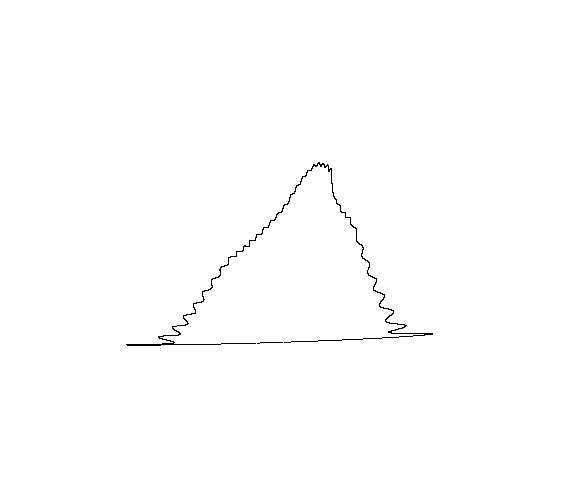
\includegraphics[width=\textwidth]{./figs/A256.png}
	        \caption{75 coeficientes}
                \label{fig:fundteor_fourier_desc_256}
        \end{subfigure}
	~ %add desired spacing between images, e. g. ~, \quad, \qquad etc.
          %(or a blank line to force the subfigure onto a new line)
	\begin{subfigure}[b]{0.29\textwidth}
                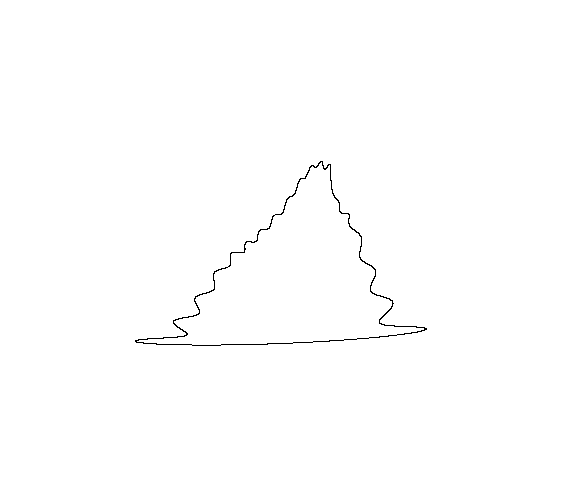
\includegraphics[width=\textwidth]{./figs/A512.png}
	        \caption{37 coeficientes}
                \label{fig:fundteor_fourier_desc_512}
        \end{subfigure}
	~ %add desired spacing between images, e. g. ~, \quad, \qquad etc.
          %(or a blank line to force the subfigure onto a new line)
	\begin{subfigure}[b]{0.29\textwidth}
                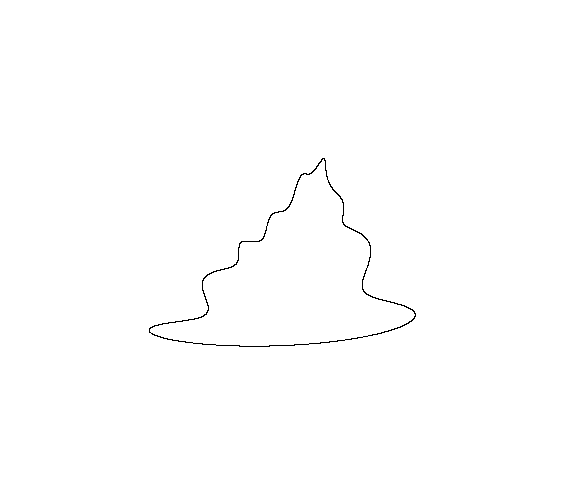
\includegraphics[width=\textwidth]{./figs/A1024.png}
	        \caption{18 coeficientes}
                \label{fig:fundteor_fourier_desc_1024}
        \end{subfigure}

	\begin{subfigure}[b]{0.29\textwidth}
                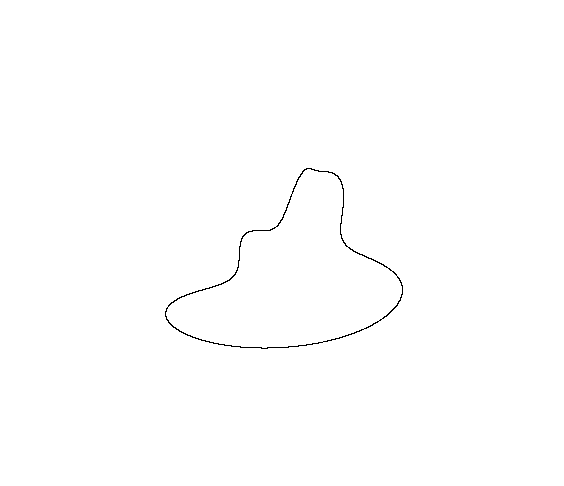
\includegraphics[width=\textwidth]{./figs/A2048.png}
	        \caption{9 coeficientes}
                \label{fig:fundteor_fourier_desc_2048}
        \end{subfigure}
	~ %add desired spacing between images, e. g. ~, \quad, \qquad etc.
          %(or a blank line to force the subfigure onto a new line)
	\begin{subfigure}[b]{0.29\textwidth}
                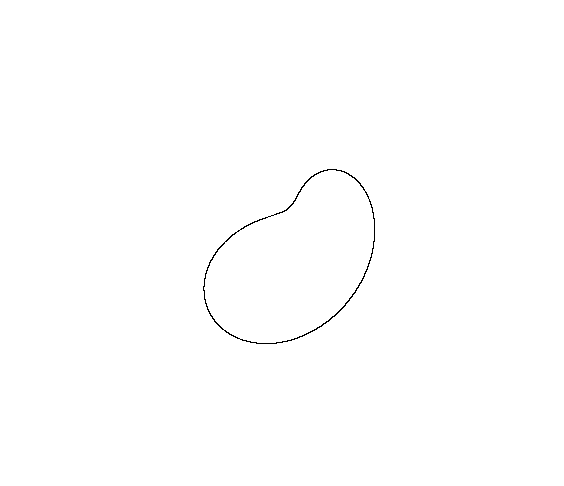
\includegraphics[width=\textwidth]{./figs/A4096.png}
	        \caption{4 coeficientes}
                \label{fig:fundteor_fourier_desc_4096}
        \end{subfigure}
	~ %add desired spacing between images, e. g. ~, \quad, \qquad etc.
          %(or a blank line to force the subfigure onto a new line)
	\begin{subfigure}[b]{0.29\textwidth}
                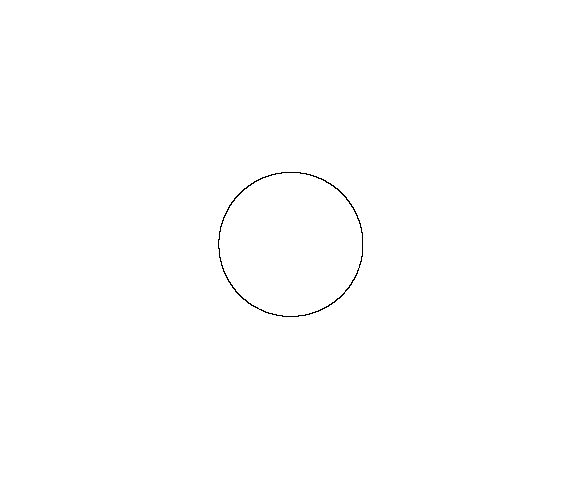
\includegraphics[width=\textwidth]{./figs/A8192.png}
	        \caption{2 coeficientes}
                \label{fig:fundteor_fourier_desc_8192}
        \end{subfigure}

        \caption{Imagem original e imagens reconstitu�das utilizando $n$ descritores de \emph{fourier}.}
	\fonte{Autoria pr�pria}
	\label{fig:fundteor_fourier_desc}
\end{figure}



\section{Classifica��o} \label{sec:classificacao}

Esta se��o apresenta uma vis�o geral de reconhecimento de padr�es utilizando redes neurais.


\subsection{Redes neurais}

Redes neurais s�o elementos n�o lineares (chamados neur�nios) interconectados da mesma maneira que se acredita que os neur�nios est�o conectados no c�rebro. Usam-se essas redes para tomadas de decis�o ap�s seus coeficientes terem sido ajustados por meio de apresenta��es sucessivas de conjuntos de dados de treinamento \cite{GONZALEZ-2006}.

Na forma mais simples no entanto a rede � um elemento linear e � composta por um �nico neur�nio, tamb�m chamado \emph{perceptron}. Esse neur�nio ent�o aprende uma fun��o linear para separar dois conjuntos de dados de treinamento linearmente separ�veis. A figura \ref{fig:fundteor_nn_perceptron_model} apresenta o modelo b�sico para um \emph{perceptron}. A resposta desse \emph{perceptron} � baseada na soma ponderada das entradas, dada pela equa��o \ref{eq:fundteor_nn_perceptron}.

\begin{equation}
d(x) = \sum_{i=1}^{n} (\omega _{i} x_{i}) + \omega _{n+1}
\label{eq:fundteor_nn_perceptron}
\end{equation}

Os coeficientes $w_{i}, i=1,2,...,n,n+1$, s�o chamados de pesos e modificam a soma antes que os valores de entrada passem pelo elemento de ativa��o, tamb�m chamado de fun��o de ativa��o. Os pesos podem ser comparados �s sinapses que ocorrem no c�rebro humano. No caso particular da figura \ref{fig:fundteor_nn_perceptron_model} a sa�da do \emph{perceptron} ser� $+1$ caso a entrada perten�a a classe $\omega_{1}$ e $-1$ caso a entrada perten�a a classe $\omega_{2}$.

\begin{figure}[H]
	\centering
	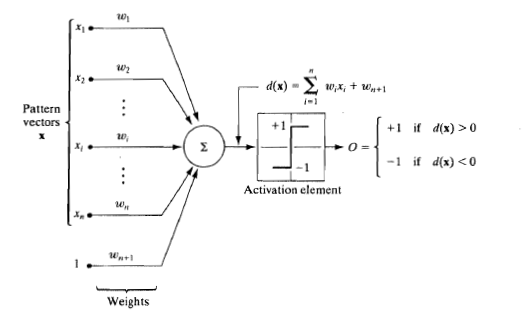
\includegraphics[width=1\textwidth]{./figs/perceptron_model.png}
	\caption{Modelo de \emph{perceptron}.}
	\fonte{\cite{GONZALEZ-2006}}
	\label{fig:fundteor_nn_perceptron_model}
\end{figure}

Esse tipo de abordagem formada por um �nico \emph{perceptron} n�o � capaz de separar mais do que duas classes e tamb�m n�o � capaz de separar classes que n�o s�o linearmente separ�veis. Isso se d� devido ao fato de que a equa��o \ref{eq:fundteor_nn_perceptron} quando expandida define um hiperplano em um espa�o $n$-dimensional.

Utilizam-se portanto para problemas mais complexos redes de neur�nios, tamb�m chamada de \emph{multi-layer perceptron} ou \emph{multi-layer feedforward network}. Cada neur�nio � formado por uma estrutura do mesmo tipo da estrutura do \emph{perceptron}, com a diferen�a de a fun��o de ativa��o ser geralmente uma fun��o sigmoide ao inv�s de um simples limiar. A fun��o sigmoide pode ser vista na equa��o \ref{eq:fundteor_nn_perceptron_sigmoide} e na figura \ref{fig:fundteor_nn_multilayer_perceptron_sigmoide}. As sa�das dos neur�nios est�o interconectadas com as entradas de outros neur�nios. Essa estrutura pode ser vista na figura \ref{fig:fundteor_nn_multilayer_perceptron_model}.

\begin{equation}
h_{j}(I_{j}) = \frac {1}{1+e^{-(I_{j} + \theta_{j})/\theta_{O}}}
\label{eq:fundteor_nn_perceptron_sigmoide}
\end{equation}

\begin{figure}[H]
	\centering
	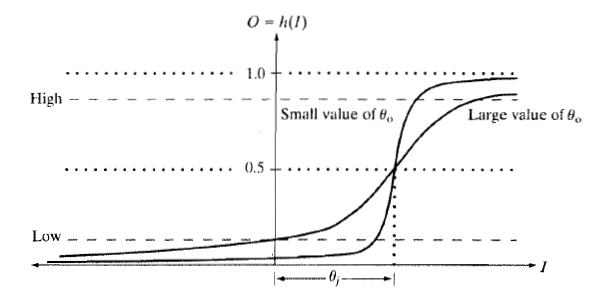
\includegraphics[width=1\textwidth]{./figs/multilayer_perceptron_sigmoide.png}
	\caption{Gr�fico da fun��o de ativa��o sigmoide.}
	\fonte{\cite{GONZALEZ-2006}}
	\label{fig:fundteor_nn_multilayer_perceptron_sigmoide}
\end{figure}

\begin{figure}[H]
	\centering
	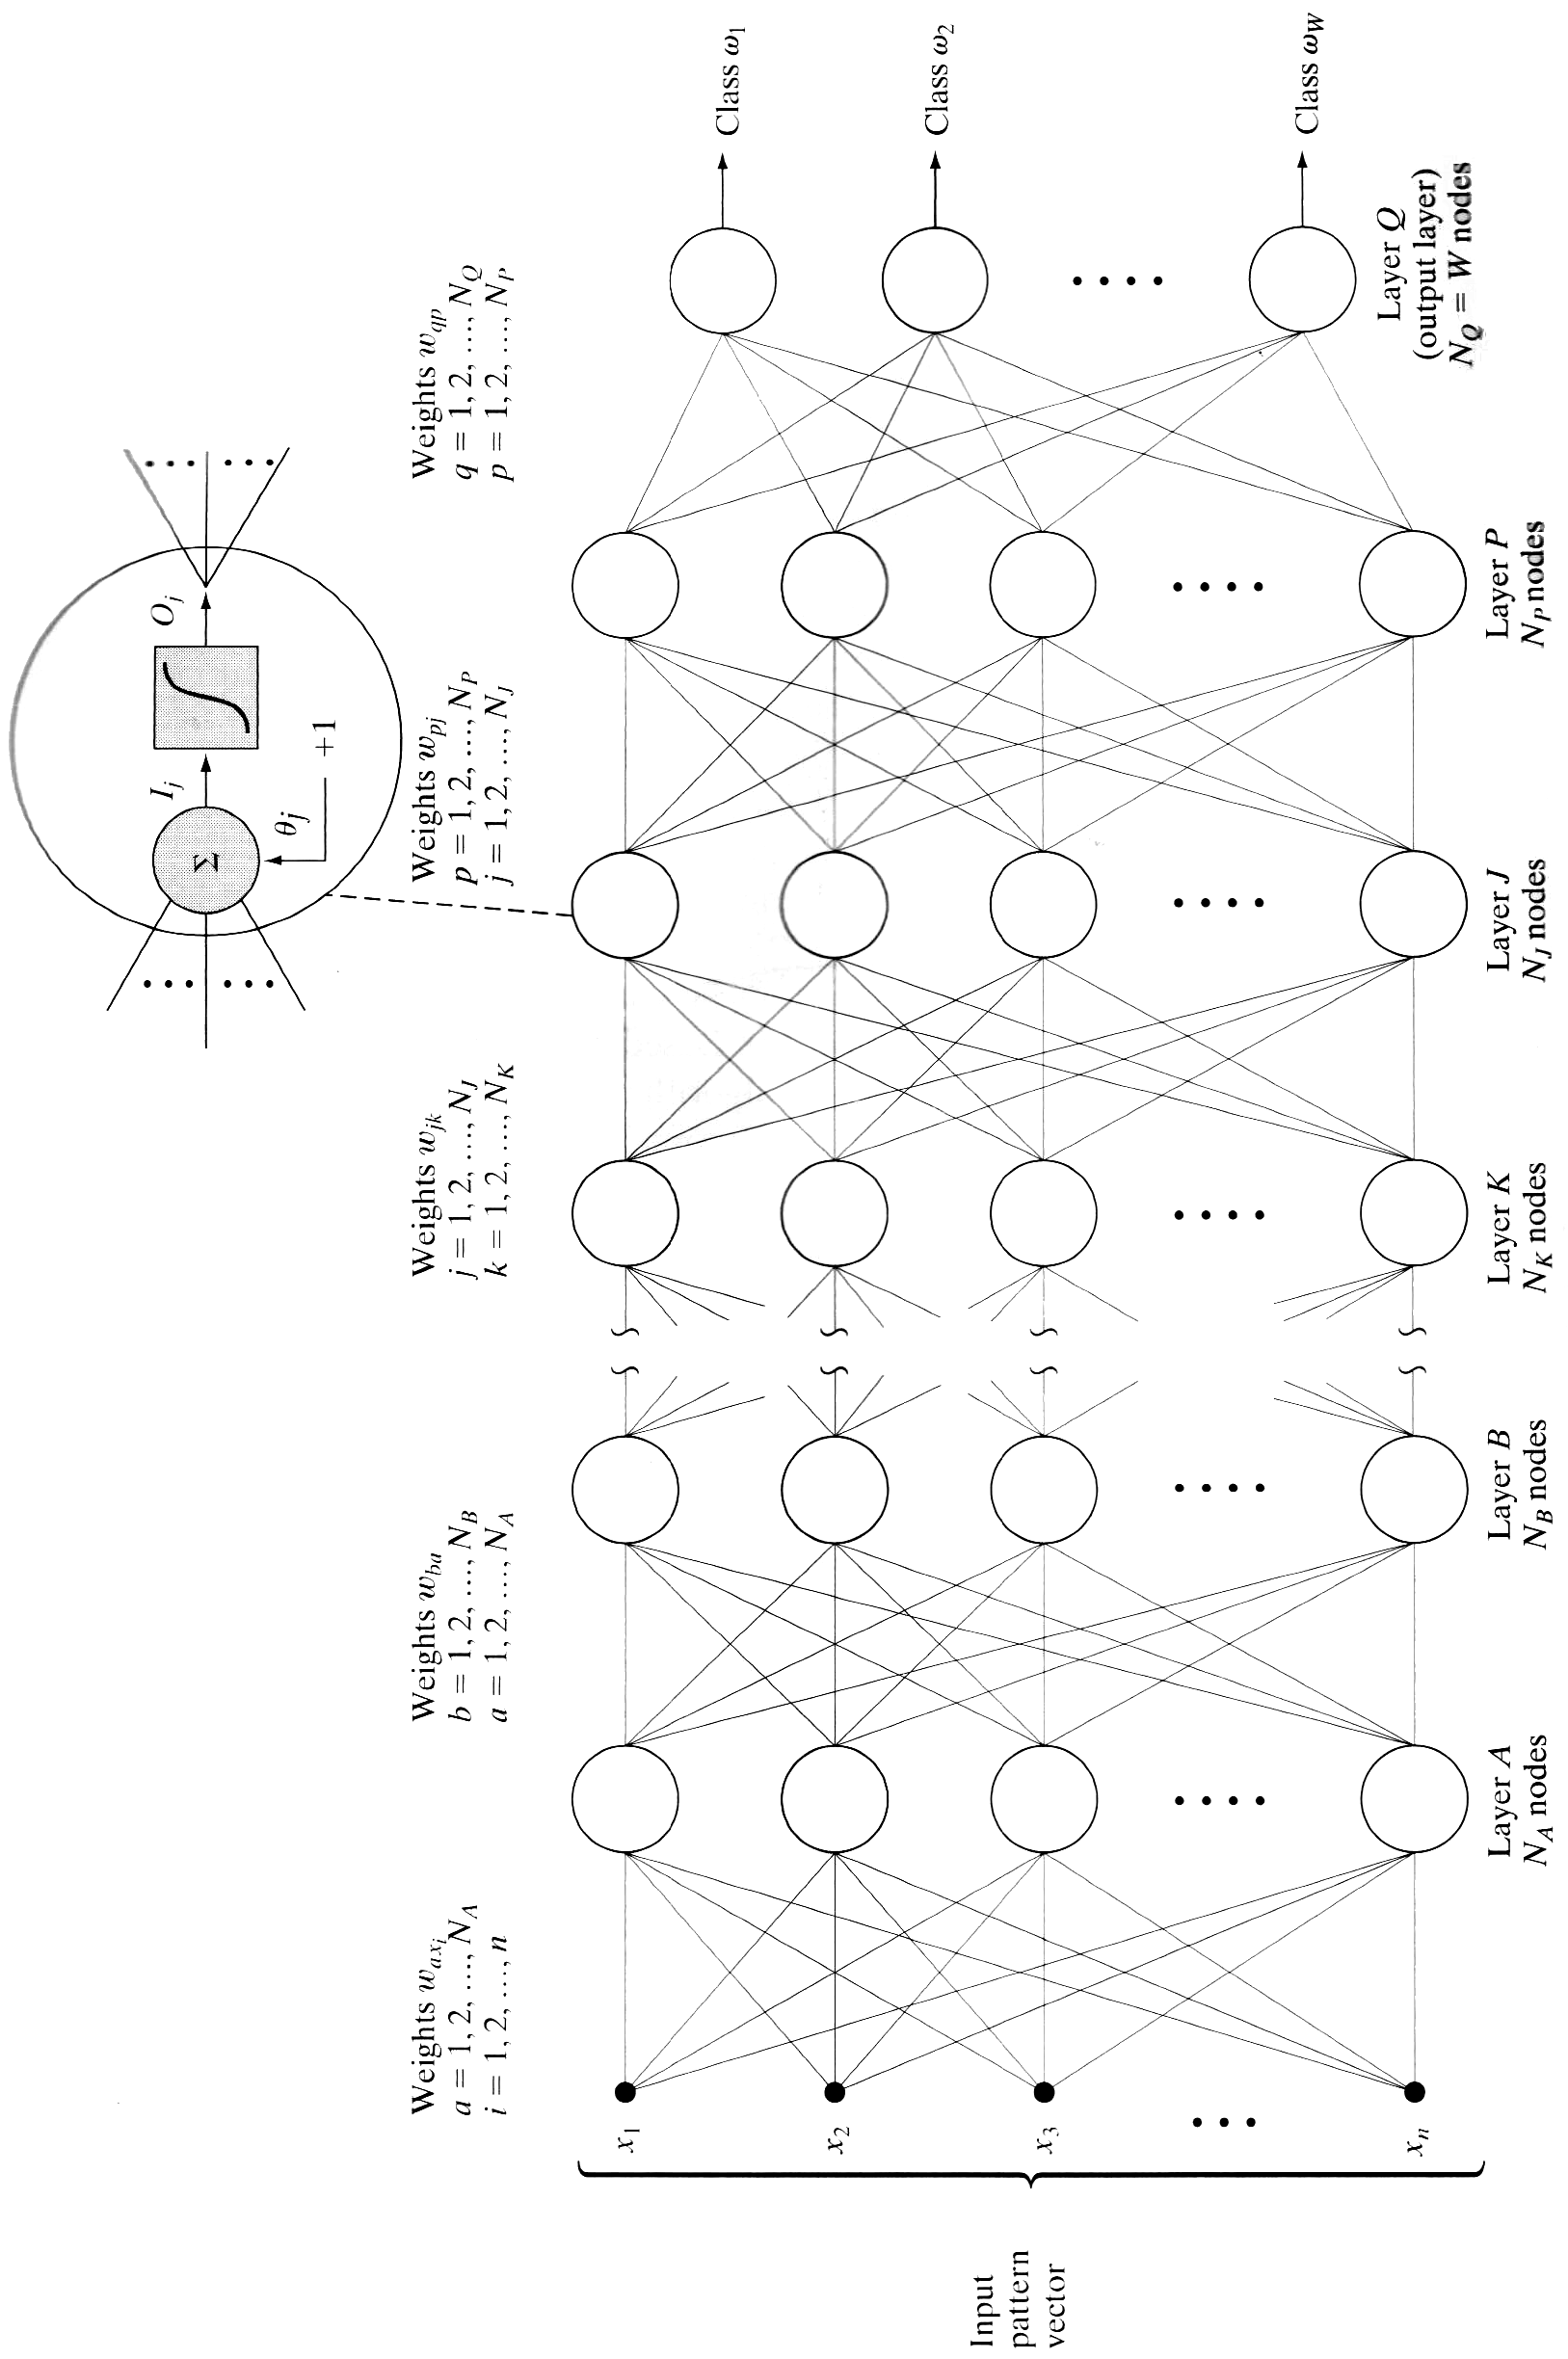
\includegraphics[width=1\textwidth]{./figs/multilayer_perceptron_model.png}
	\caption{Modelo de \emph{multi-layer feedforward network}.}
	\fonte{\cite{GONZALEZ-2006}}
	\label{fig:fundteor_nn_multilayer_perceptron_model}
\end{figure}

Nesse tipo de rede a primeira camada, $A$, possui o mesmo n�mero de neur�nios que a dimens�o do vetor descritor da entrada, $N_{A} = n$. Semelhantemente o n�mero de neur�nios da camada de sa�da, $Q$, � igual ao n�mero de classes que a rede deve reconhecer, $N_{Q} = {W}$. A rede reconhece uma entrada como sendo parte de uma classe quando a sa�da da classe � um e as demais sa�das s�o zero.

Pode-se demonstrar que redes desse tipo s�o capazes de separar regi�es convexas no espa�o $n$-dimensional de entradas utilizando duas camadas de neur�nios. S�o tamb�m capazes de separar classes em regi�es arbitr�rias utilizando tr�s camadas de neur�nios  \cite{GONZALEZ-2006}. A complexidade das regi�es separadas por uma rede de tr�s camadas se d� pelo n�mero de neur�nios em cada camada. Isso est� resumido na figura \ref{fig:fundteor_nn_multilayer_perceptron_decision}.

\begin{figure}[H]
	\centering
	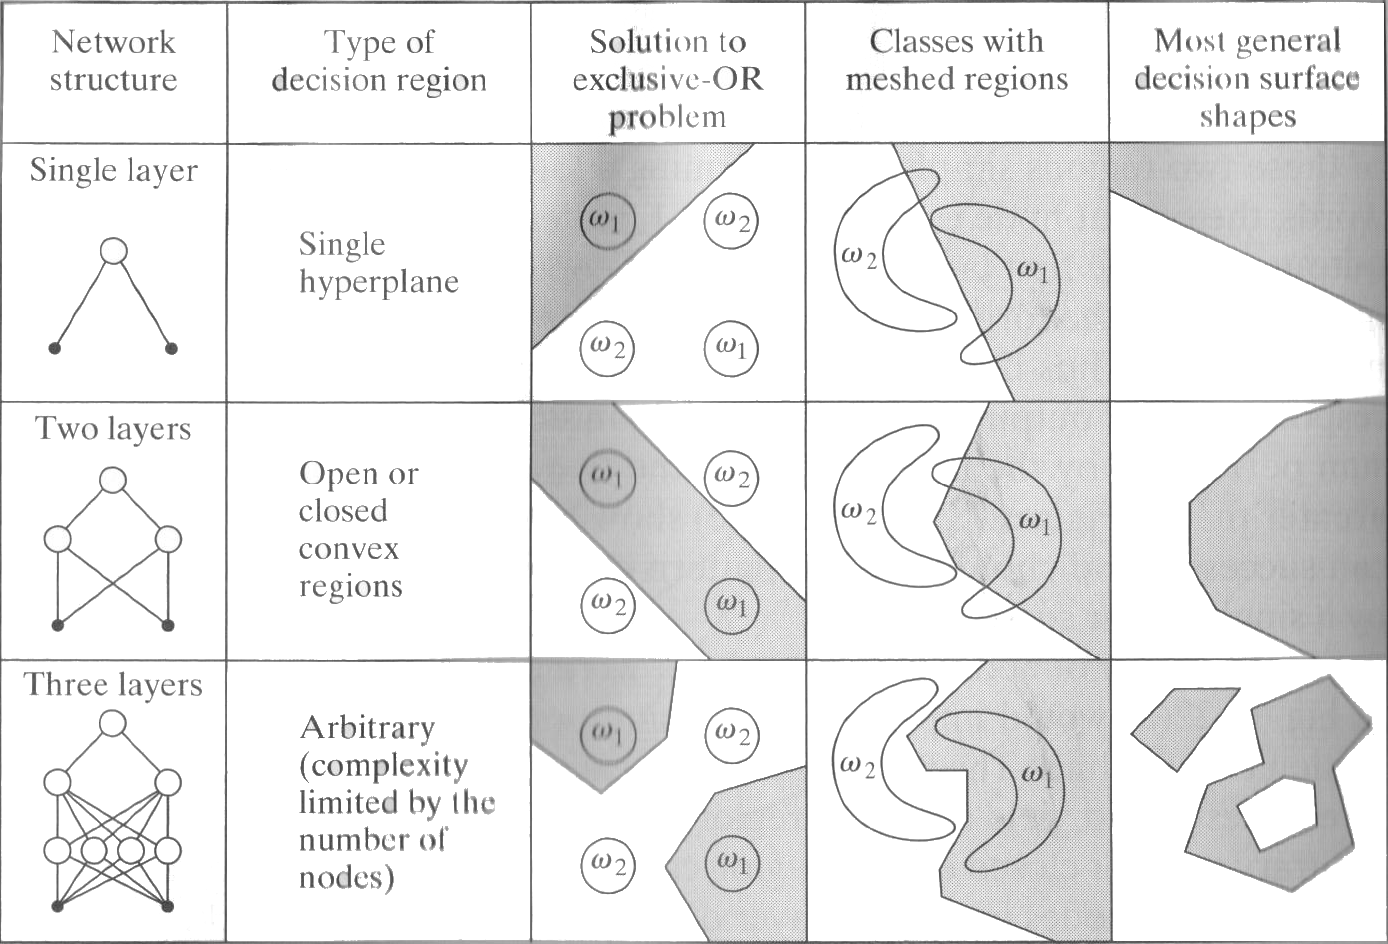
\includegraphics[width=1\textwidth]{./figs/multilayer_perceptron_decision.png}
	\caption{Estruturas de redes neurais e sua respectiva capacidade de decis�o.}
	\fonte{\cite{GONZALEZ-2006}}
	\label{fig:fundteor_nn_multilayer_perceptron_decision}
\end{figure}


\subsubsection{Treinamento de \emph{perceptrons}}

O treinamento de \emph{perceptrons} consiste em determinar os valores adequados de $\omega_{i}$ para que a soma ponderada das entradas forme a sa�da adequada para a fun��o de ativa��o. Existem diversos m�todos de treinamento para determinar os valores de $\omega_{i}$ para um �nico perceptron. Apresenta-se a seguir o m�todo denominado \emph{delta rule} ou \emph{least-mean-square}.

A principal caracter�stica do m�todo \emph{delta rule} � que ele minimiza o erro entre a sa�da desejada e a sa�da real do \emph{perceptron} em cada passo de treinamento. Considere a fun��o da equa��o \ref{eq:fundteor_nn_perceptron_error}. 

\begin{equation}
J(w) = \frac{1}{2} (r - w^{T}y)^2
\label{eq:fundteor_nn_perceptron_error}
\end{equation}

$J(w)$ representa o erro quadr�tico para um dado conjunto de pesos $w$. O erro � calculado como sendo a diferen�a entre a sa�da desejada do \emph{perceptron} $r$ e a sa�da real dada pelo produto do vetor de pesos transposto $w^{T}$ com o valor de entrada do conjunto de treinamento $y$.

O objetivo do treinamento pelo m�todo \emph{delta rule} � minimizar $J(w)$ ajustando os valores dos pesos $w$.

Se $w(k)$ representa o vetor de pesos no passo de treinamento $k$, ent�o pode-se calcular $w(k+1)$ de forma a reduzir o valor de $J(w)$ utilizando a equa��o \ref{eq:fundteor_nn_perceptron_error_desc} \cite{GONZALEZ-2006}.

\begin{equation}
w(k+1) = w(k) - \alpha \left [ \frac{\partial J(w)}{\partial w} \right ] _{w=w(k)}
\label{eq:fundteor_nn_perceptron_error_desc}
\end{equation}

Onde $\alpha > 0$ � uma constante escolhida de acordo com o grau de corre��o que se deseja a cada passo. Da equa��o \ref{eq:fundteor_nn_perceptron_error} tem se que:

\begin{equation}
\frac{\partial J(w)}{\partial w} = -(r - w^{T} y)y
\label{eq:fundteor_nn_perceptron_error_der}
\end{equation}

Substituindo a equa��o \ref{eq:fundteor_nn_perceptron_error_der} na equa��o \ref{eq:fundteor_nn_perceptron_error_desc} resulta na equa��o \ref{eq:fundteor_nn_perceptron_error_desc_2} que pode ser utilizada para o c�lculo dos coeficientes $w(k+1)$ dados os coeficientes $w(k)$, a sa�da desejada $r$ e o valor de entrada do conjunto de treinamento $y$. 

\begin{equation}
w(k+1) = w(k) + \alpha \left [ r(k) - w^{T} (k) y(k) \right ] y(k)
\label{eq:fundteor_nn_perceptron_error_desc_2}
\end{equation}

Pode-se demonstrar que utilizando esse m�todo para calcular os coeficientes, tem-se a redu��o do erro do $perceptron$ em um fator de $\alpha y(k)^{T} y(k)$ a cada ciclo de treinamento \cite{GONZALEZ-2006}.

\subsubsection{Treinamento de \emph{multi-layer perceptrons}}

O treinamento de redes multicamadas pode ser efetuado de maneira semelhante ao treinamento de um �nico \emph{perceptron}. Considere a equa��o \ref{eq:fundteor_nn_perceptron_error_multi}. O erro quadr�tico $E_{Q}$ obtido na camada de sa�da � dado pela soma dos erros quadr�ticos em todos os \emph{perceptrons} da camada de sa�da (\emph{perceptrons} de $1$ a $N_{Q}$). O erro em cada \emph{perceptron} � dado pela diferen�a entre a sa�da desejada $r_{q}$, no perceptron $q$, e a sa�da obtida $O_{q}$.

\begin{equation}
E_{Q} = \frac{1}{2} \sum_{q=1}^{N_{Q}} (r_{q} - O_{q})^{2}
\label{eq:fundteor_nn_perceptron_error_multi}
\end{equation}

Novamente deseja-se minimizar o erro $E_{Q}$ em cada passo de treinamento. Minimizando a equa��o \ref{eq:fundteor_nn_perceptron_error_multi} chega-se a dois casos. O primeiro � quando o \emph{perceptron} est� na �ltima camada da rede. Nesse casos sabe-se o valor esperando na sa�da do perceptron, que � dado por $O_{q}$. Por outro lado quando o \emph{perceptron} est� em uma camada intermedi�ria � necess�rio que primeiro se defina o erro em fun��o de par�metros conhecidos na rede. Esse processo foi desenvolvido por \cite{GONZALEZ-2006} e a seguir apresenta-se o resultado.

Para \emph{perceptrons} na camada de sa�da $Q$ os pesos $w(k+1)$ podem ser calculado pelas equa��es \ref{eq:fundteor_nn_perceptron_error_multi_desc_2} e \ref{eq:fundteor_nn_perceptron_error_multi_desc_3}. $K$ � a camada que precede a camada de sa�da $Q$.

\begin{equation}
w_{q}(k+1) = w_{q}(k) + \alpha \delta_{q} O_{K}
\label{eq:fundteor_nn_perceptron_error_multi_desc_2}
\end{equation}

\begin{equation}
\delta_{q} =  (r_{q}-O_{q}) h'_{q}(I_{q})
\label{eq:fundteor_nn_perceptron_error_multi_desc_3}
\end{equation}

Onde:

\begin{itemize}
\item $w_{q}(k+1)$ s�o os pesos atualizados do \emph{perceptron} $q$;
\item $w_{q}(k)$ s�o os pesos antigos do \emph{perceptron} $q$;
\item $\alpha > 0$ � uma constante escolhida de acordo com o grau de corre��o que se deseja a cada passo;
\item $O_{K}$ s�o as sa�das dos \emph{perceptrons} da camada $K$;
\item $r_{q}$ � a sa�da esperada do \emph{perceptron}, dada pelo conjunto de treinamento;
\item $O_{q}$ � a sa�da atual no \emph{perceptron} $q$;
\item $h'_{q}(I_{q})$ � a derivada da fun��o de ativa��o do \emph{perceptron} $q$ para a entrada $I_{q}$.
\end{itemize}

Para \emph{perceptrons} em uma camada intermedi�ria $J$, onde a camada seguinte � a camada $P$ e a camada antecedente � a camada $K$, os pesos $w(k+1)$ podem ser calculados pelas equa��es \ref{eq:fundteor_nn_perceptron_error_multi_desc_4} e \ref{eq:fundteor_nn_perceptron_error_multi_desc_5}.

\begin{equation}
w_{j}(k+1) = w_{j}(k) + \alpha \delta_{j} O_{K}
\label{eq:fundteor_nn_perceptron_error_multi_desc_4}
\end{equation}

\begin{equation}
\delta_{j} =  h'_{j}(I_{j}) \sum_{p=1}^{N_{P}} \delta _{P} \omega _{jp}
\label{eq:fundteor_nn_perceptron_error_multi_desc_5}
\end{equation}

Onde:

\begin{itemize}
\item $w_{j}(k+1)$ s�o os pesos atualizados do \emph{perceptron} $j$;
\item $w_{j}(k)$ s�o os pesos antigos do \emph{perceptron} $j$;
\item $\alpha > 0$ � uma constante escolhida de acordo com o grau de corre��o que se deseja a cada passo;
\item $O_{K}$ s�o as sa�das dos \emph{perceptrons} da camada $K$;
\item $h'_{j}(I_{j})$ � a derivada da fun��o de ativa��o para a entrada $I_{j}$;
\item $p$ at� $N_{P}$ s�o todos os \emph{perceptrons} da camada $P$;
\item $\delta _{P}$ � o valor de $\delta$ que havia sido calculado para o perceptron $p$ da camada $P$ quando os pesos da camada $P$ foram atualizados.
\item $\omega _{jp}$ � o valor do peso $\omega$ que havia sido calculado para o \emph{perceptron} $j$ em cada perceptron da camada $P$.
\end{itemize}

Caso a fun��o de ativa��o escolhida seja a fun��o sigmoide da equa��o \ref{eq:fundteor_nn_perceptron_sigmoide}, com $\theta_{O} = 1$, pode-se demonstrar que $h'_{j}(I_{j})$ assume o valor da equa��o \ref{eq:fundteor_nn_perceptron_sigmoide_der} e semelhantemente $h'_{q}(I_{q})$ assume o valor da equa��o \ref{eq:fundteor_nn_perceptron_sigmoide_der2} \cite{GONZALEZ-2006}.

\begin{equation}
h'_{j}(I_{j}) = O_{j}(1-O_{j});
\label{eq:fundteor_nn_perceptron_sigmoide_der}
\end{equation}

Onde:
\begin{itemize}
\item $O_{j}$ � a sa�da atual no \emph{perceptron} $j$;
\end{itemize}

\begin{equation}
h'_{q}(I_{q}) = O_{q}(1-O_{q});
\label{eq:fundteor_nn_perceptron_sigmoide_der2}
\end{equation}

Onde:
\begin{itemize}
\item $O_{q}$ � a sa�da atual no \emph{perceptron} $q$;
\end{itemize}

Como se pode ver � necess�rio iniciar o processo de atualiza��o dos pesos da rede pela camada de sa�da. Na camada de sa�da da rede � o �nico lugar onde se sabe qual � a sa�da que cada \emph{perceptron} deveria ter. Para as camadas antecedentes a atualiza��o deve ser feita em fun��o dessas sa�das. Portanto cada camada depende de par�metros da camada seguinte na rede. Esse processo de atualiza��o dos pesos iniciando pela ultima camada e voltando at� a primeira recebe o nome de \emph{back propagation}. O m�todo mencionado anteriormente recebe o nome de \emph{delta rule}, no entanto existem diversos m�todos diferentes mas que utilizam a mesma estrat�gia de propaga��o das corre��es na rede. Todos esses m�todos s�o classificados como m�todos de \emph{back propagation}.



%---------- Segundo Capitulo ----------
\chapter{Desenvolvimento} \label{chap:desenv}

Este cap�tulo apresenta o desenvolvimento do projeto, detalhando cada parte do sistema desenvolvido. A descri��o apresentada a seguir referencia os conceitos apresentados no cap�tulo \ref{chap:fundteor}. O sistema foi implementado no software Matlab \cite{MATLAB} permitindo a execu��o de diversos testes para valida��o conforme ser� visto no capitulo \ref{chap:testes}. A figura \ref{fig:desenv_overview} apresenta uma vis�o geral do sistema desenvolvido.

\begin{figure}[H]
	\centering
	\includegraphics[width=1\textwidth]{./figs/visao_geral.jpg}
	\caption{Vis�o geral do sistema desenvolvido.}
	\fonte{Autoria pr�pria}
	\label{fig:desenv_overview}
\end{figure}

O capitulo divide-se em sete se��es. As primeiras seis se��es apresentam com detalhes os blocos da figura \ref{fig:desenv_overview}: A se��o \ref{sec:desenv_seg1} e a se��o \ref{sec:desenv_seg2} mostram como os conceitos da se��o \ref{sec:segmentacao} foram aplicados para segmentar a imagem capturada. A se��o \ref{sec:desenv_desc1} e a se��o \ref{sec:desenv_desc2} apresentam como os descritores de \emph{fourier} e as propriedades estudados na se��o \ref{subsec:propriedades} foram aplicados para formar um descritor para as imagens. As se��es \ref{sec:desenv_class1} e \ref{sec:desenv_class2} apresentam como os descritores foram utilizados para classificar e determinar o �ngulo das imagens. Finalmente, na se��o \ref{sec:desenv_consideracoes}, algumas considera��es sobre o desenvolvimento do projeto s�o apresentadas.


\section{Segmenta��o: etapa 1} \label{sec:desenv_seg1}

A primeira etapa da segmenta��o consiste em uma s�rie de limiariza��es e filtros para localizar a regi�o de interesse na imagem. A sa�da da primeira etapa � uma imagem bin�ria contendo a regi�o de interesse. O processo da primeira etapa pode ser visto na figura \ref{fig:desenv_seg1}.

O processo inicia pela subtra��o da imagem RGB de fundo da imagem RGB com o objeto. Como resultado tem-se uma imagem RGB contendo as diferen�as inseridas pelo objeto na imagem. Para n�o perder informa��es intr�nsecas da imagem RGB no processo de convers�o para escala de cinza dividem-se os canais R, G e B da imagem. Cada canal � processado separadamente. Primeiramente os canais s�o limiarizados utilizando o m�todo global de \emph{Otsu}, discutido na se��o \ref{sub:fundteor_limiarizacao}. Em seguida os canais s�o submetidos � opera��o morfol�gica de fechamento, vista na se��o \ref{sub:fundteor_op_morfologicas}. A opera��o de fechamento � aplicado para reduzir o ruido do tipo pimenta (pixeis pretos espalhados aleatoriamente pela imagem). Na sequencia os tr�s canais processados separadamente s�o unidos atrav�s da opera��o l�gica OU para formar uma �nica imagem. Finalmente a maior regi�o conexa da imagem � selecionada para ser a regi�o de interesse.

Embora n�o se possa ver visualmente nenhum progresso significativo em alguns passos da sequencia de imagens da figura \ref{fig:desenv_seg1}, a primeira etapa da segmenta��o necessita de todos eles. Todos os passos apresentados anteriormente garantem a robustez do sistema, fornecendo a regi�o de interesse para a etapa seguinte.

\begin{figure}[H]
	\centering
	\includegraphics[width=0.8\textwidth]{./figs/segmentacao_1.jpg}
	\caption{Primeira etapa da segmenta��o.}
	\fonte{Autoria pr�pria}
	\label{fig:desenv_seg1}
\end{figure}


\section{Segmenta��o: etapa 2} \label{sec:desenv_seg2}

A segunda etapa da segmenta��o � respons�vel por normalizar a imagem. Esta etapa recebe como entrada a regi�o de interesse e apresenta como sa�da duas op��es de normaliza��o, al�m de um autovetor e seu oposto. O processo pode ser visto na figura \ref{fig:desenv_seg2}.

\begin{figure}[H]
	\centering
	\includegraphics[width=0.9\textwidth]{./figs/segmentacao_2.jpg}
	\caption{Segunda etapa da segmenta��o.}
	\fonte{Autoria pr�pria}
	\label{fig:desenv_seg2}
\end{figure}

A regi�o de interesse obtida da primeira etapa de segmenta��o � esqueletonizada e podada pelos processos descritos na se��o \ref{sub:fundteor_esqueletonizacao}. Em seguida o processo de normaliza��o da se��o \ref{sub:fundteor_normalizacao} � aplicado.

Como dito na se��o \ref{sub:fundteor_normalizacao}, o autovetor associado ao maior autovalor da matriz de covari�ncias aponta na dire��o de maior varia��o dos dados. Por�m o autovetor n�o aponta no sentido de maior varia��o dos dados. Empiricamente percebe-se que o autovetor aponta sempre no sentido positivo dos eixos da imagem. Esse comportamento leva a duas poss�veis normaliza��es para cada imagem. A normaliza��o obtida utilizando o autovetor $A$ e a normaliza��o pelo oposto do autovetor, $A'=-A$. 

Essas duas op��es de normaliza��o s�o ent�o apresentadas a etapa seguinte juntamente com os respectivos autovetores.


\section{Descri��o: etapa 1} \label{sec:desenv_desc1}

Essa etapa de descri��o � respons�vel por gerar um descritor para a imagem normalizada utilizando o autovetor $A$ (chamada mais adiante de imagem pr�-normalizada). A imagem normalizada utilizando o autovetor $A'$ n�o � utilizada. A figura \ref{fig:desenv_desc1} resume o processo desta etapa.

O descritor � composto por 20 descritores de \emph{fourier}, $d1,d2,...,d20$, concatenados com 9 propriedades b�sicas da imagem, $p1,p2,...,p9$. A tabela \ref{tab:descritores-etapa1} detalha o descritor gerado.

\begin{figure}[H]
	\centering
	\includegraphics[width=0.9\textwidth]{./figs/descricao_1.jpg}
	\caption{Primeira etapa da descri��o.}
	\fonte{Autoria pr�pria}
	\label{fig:desenv_desc1}
\end{figure}

\begin{table}[htb!]
	\centering
	\caption[Descritor para primeira etapa]{Descritor para primeira etapa.}		
	\begin{tabular}[H]{ l l l l }
	  \hline
	  Descritor & Descri��o \\
	  \hline
	  $d1 ... d20$ & 20 descritores de \emph{fourier} \\
	  $p1$ & �rea \\
	  $p2$ & �rea convexa \\
	  $p3$ & Excentricidade \\
	  $p4$ & N�mero de Euler \\
	  $p5$ & Extens�o \\
	  $p6$ & �rea preenchida \\
	  $p7$ & Tamanho do eixo principal \\
	  $p8$ & Tamanho do eixo secund�rio \\
	  $p9$ & Solidez \\
	  \hline  	
	\end{tabular}
	\fonte{Autoria pr�pria}
	\label{tab:descritores-etapa1}
\end{table}


\section{Classifica��o} \label{sec:desenv_class1}

A fun��o da etapa de classifica��o � tomar como entrada o descritor da imagem pr�-normalizada e fornecer como sa�da a classe a qual o objeto da imagem pertence. Al�m disso � respons�vel por dizer qual a normaliza��o correta para a imagem. Ou seja, se a imagem normalizada corretamente utiliza o autovetor $A$ ou o oposto $A'$. Esse processo � mostrado na figura \ref{fig:desenv_class1}.

Para essa tarefa foi utilizada uma rede neural pois ela fornece um m�todo de classifica��o baseado em treinamento onde n�o � necess�rio que se tenha conhecimento pr�vio das propriedades estat�sticas de cada classe de padr�es \cite{GONZALEZ-2006}. A rede utilizada � formada por duas camadas, 29 entradas e $2N$ sa�das. Onde $N$ � o n�mero de classes a serem identificadas pelo sistema. A primeira camada possui 20 \emph{perceptrons} e a camada de sa�da possui $2N$ perceptrons.
O n�mero de \emph{perceptrons} na primeira camada foi escolhido empiricamente. O n�mero de sa�das � $2N$ pois a rede deve ser capaz de identificar imagens normalizadas pelo autovetor $A$ e imagens normalizadas pelo oposto $A'$. A fun��o de ativa��o para as duas camadas � a fun��o sigmoide vista na se��o \ref{subsec:fundteor_redes_neurais}. A fun��o sigmoide � uma boa escolha para redes de classifica��o pois possui uma transi��o r�pida entre -1 e 1 para entradas de $-\infty$ a $+\infty$ \cite{MATHWORKS-HELP-3}.

Para formar o conjunto de treinamento da rede � necess�rio que se obtenha amostras de imagens com as respectivas classes.  Em seguida deve-se executar todos os passos at� obter as duas possibilidades de normaliza��o de cada imagem, e os descritores tomando a normaliza��o dada pelo autovetor $A$. O descritor � ent�o fornecido como entrada da rede e a sa�da da rede � dada pelo autovetor que leva a normaliza��o correta da imagem. Por exemplo, se a normaliza��o correta da classe $n$ � dada pelo autovetor $A$, a posi��o $2n$ da sa�da � um e o restante zero. Se a normaliza��o correta � dada pelo oposto do autovetor, $A'$, ent�o a posi��o "2n+1" � um e o restante zero. Esse �ltimo passo necessita ser executado manualmente para que se possa "ensinar" a rede qual a normaliza��o correta para cada classe.

A rede � treinada utilizando um algoritmo de \emph{back propagation} conforme visto na se��o \ref{subsec:fundteor_redes_neurais}. O algoritmo utilizado para esta rede em espec�fico utiliza o m�todo chamado \emph{Bayesian regularization}. O m�todo em quest�o n�o � aprofundado aqui. A escolha foi baseada na documenta��o presente em \cite{MATHWORKS-HELP-4} que afirma que redes treinadas utilizando essa otimiza��o possuem boa capacidade de generaliza��o.

\begin{figure}[H]
	\centering
	\includegraphics[width=0.9\textwidth]{./figs/classificacao_1.jpg}
	\caption{Etapa de classifica��o.}
	\fonte{Autoria pr�pria}
	\label{fig:desenv_class1}
\end{figure}


\section{Descri��o: etapa 2} \label{sec:desenv_desc2}

A segunda etapa da descri��o recebe como entrada a imagem normalizada pelo autovetor correto. A fun��o desta etapa � gerar um descritor para a imagem normalizada, que auxiliar� na etapa de estimativa do �ngulo do objeto.

Tanto esta etapa, quanto a estimativa de �ngulo descrita na pr�xima se��o, seriam desnecess�rias em ambientes ideais. Veja por exemplo as imagens da figura \ref{fig:desenv_desc3}. Todas as imagens foram obtidas para um mesmo objeto, sujeito �s mesmas condi��es gerais, mas em rota��es diferentes. Mudan�as pequenas, como ru�do ou pequenas diferen�as na ilumina��o, influenciaram a dire��o do autovetor calculado produzindo resultados diferentes.

\begin{figure}[H]
	\centering
	\includegraphics[width=0.9\textwidth]{./figs/normalizacoes_A.png}
	\caption{Imagens normalizadas para diferentes entradas do mesmo objeto.}
	\fonte{Autoria pr�pria}
	\label{fig:desenv_desc3}
\end{figure}

A diferen�a entre o autovetor calculado para cada caso � tratada na etapa de estimativa de �ngulo que recebe como entrada o descritor calculado aqui. O descritor portanto deve conter informa��es relacionadas � posi��o do objeto na imagem normalizada. Utilizou-se para essa tarefa um descritor contendo 10 descritores de \emph{fourier} juntamente com as coordenadas do centroide da imagem. O descritor pode ser visto na figura \ref{fig:desenv_desc2}. 

\begin{figure}[H]
	\centering
	\includegraphics[width=0.9\textwidth]{./figs/descricao_2.jpg}
	\caption{Segunda etapa da descri��o.}
	\fonte{Autoria pr�pria}
	\label{fig:desenv_desc2}
\end{figure}

\section{Estimativa de �ngulo} \label{sec:desenv_class2}

Finalmente a �ltima etapa recebe como entrada um descritor da imagem normalizada, a classe a qual pertence o objeto e o autovetor utilizado na normaliza��o. O objetivo dessa etapa � fornecer o �ngulo de rota��o do objeto na imagem.

Considere a figura \ref{fig:desenv_class3}. Os eixos $x,y$ s�o as coordenadas da imagem. O eixo $x'$ � o eixo que foi assumido como sendo o zero para o objeto da figura. $A$ � o autovetor calculado na etapa de normaliza��o. Pela figura tem-se ent�o a equa��o \ref{eq:desenv_beta}.

\begin{equation}
\beta = \alpha - k
\label{eq:desenv_beta}
\end{equation}

Onde:

\begin{itemize}
\item $\beta$ � o �ngulo entre as coordenadas da imagem e o zero do objeto. Ou seja, o valor que se deseja obter;
\item $\alpha$ � o �ngulo dado pelo autovetor;
\item $k$ � a diferen�a entre o �ngulo do autovetor e o zero do objeto. Este valor pode variar de normaliza��o para normaliza��o, conforme visto na figura \ref{fig:desenv_desc3}.
\end{itemize}

\begin{figure}[H]
	\centering
	\includegraphics[width=0.9\textwidth]{./figs/classificacao_3.jpg}
	\caption{Representa��o do autovetor (em vermelho), dos eixos da imagem (em amarelo) e do eixo do objeto (em azul).}
	\fonte{Autoria pr�pria}
	\label{fig:desenv_class3}
\end{figure}

� necess�rio portanto determinar o valor de $k$ para cada imagem normalizada. Utilizou-se para essa tarefa uma segunda rede neural. Essa rede recebe como entrada um descritor da imagem normalizada e informa na sa�da o valor de $k$. Para cada classe � gerada uma rede diferente, visto que as varia��es s�o diferentes de classe para classe. Ap�s obter o valor $k$ da rede basta utilizar a equa��o \ref{eq:desenv_beta} para determinar o �ngulo $\beta$ do objeto. Esse processo est� resumido na figura \ref{fig:desenv_class2}.

\begin{figure}[H]
	\centering
	\includegraphics[width=0.9\textwidth]{./figs/classificacao_2.jpg}
	\caption{Segunda etapa da classifica��o.}
	\fonte{Autoria pr�pria}
	\label{fig:desenv_class2}
\end{figure}

Foi escolhida uma rede neural para essa tarefa pois assumindo que redes neurais mostram bons resultados para aproxima��o de fun��es \cite{MATHWORKS-HELP-6}, sup�s-se que tamb�m geram bons resultados para o problema exposto. A rede utilizada nessa etapa possui duas camadas, 12 entradas e uma sa�da. A primeira camada � formada por 7 \emph{perceptrons}. A melhor quantidade de perceptrons foi determinada empiricamente. A sa�da da rede possui um �nico perceptron pois a �nica sa�da da rede � o valor de $k$. A fun��o de ativa��o da primeira camada da rede � a sigmoide pois permite o aprendizado de n�o linearidades. A segunda camada da rede possui uma fun��o linear, $y=x$, favorecendo uma ampla faixa de valores de sa�da para $k$ \cite{MATHWORKS-HELP-3}.

Para o processo de treinamento da rede s�o utilizadas as mesmas amostras que foram utilizadas para o treinamento da rede respons�vel pela classifica��o do objeto. Em seguida s�o executadas as etapas descritas nas se��es anteriores at� a obten��o do descritor de entrada da rede. Al�m disso � necess�rio o conhecimento do �ngulo em que o objeto se encontra para o c�lculo de $k$ pela equa��o \ref{eq:desenv_beta}. Uma vez tendo o valor de $k$ e o descritor de entrada � poss�vel treinar a rede.

A rede � treinada utilizando um algoritmo de \emph{back propagation} conforme visto na se��o \ref{subsec:fundteor_redes_neurais}. O algoritmo utilizado para esta rede em espec�fico utiliza a otimiza��o de \emph{Levenberg-Marquardt}. A escolha foi baseada na documenta��o presente em \cite{MATHWORKS-HELP-5} que afirma que esta deveria ser a primeira op��o de treinamento para qualquer rede devido a alta velocidade de converg�ncia no treinamento.

\section{Considera��es} \label{sec:desenv_consideracoes}

Exp�s-se nesse cap�tulo a arquitetura do sistema desenvolvido. Inicialmente foi mostrado como a imagem de entrada foi segmentada utilizando t�cnicas de subtra��o de fundo, limiariza��o, filtros morfol�gicos, opera��es l�gicas e sele��o de maior regi�o. Foi mostrado tamb�m como a imagem foi descrita utilizando propriedades de regi�es e descritores de \emph{fourier}. E finalmente como os descritores foram aplicados nas redes neurais obtendo assim a classe dos objetos e a respectiva orienta��o.

Embora tenha sido apresentado apenas a arquitetura final do sistema, ao longo do desenvolvimento do projeto diversas arquiteturas foram utilizadas. A cada ciclo de desenvolvimento da metodologia em espiral adotada novos algoritmos foram acrescentados, substitu�dos ou otimizados.

% fechamento com relacao aos objetivos do capitulo
% deve ser parte da conclusao final
% podem aparecer consideracoes pessoais

\chapter{Testes e An�lise de Resultados} \label{chap:testes}

Este capitulo apresenta o ambiente de testes desenvolvido para validar o sistema, os testes efetuados e os resultados obtidos.
A se��o \ref{sec:testes_ambiente} apresenta um ambiente de testes, que possibilita a captura de imagens de forma automatizada e os objetos utilizados para valida��o do sistema. Em seguida, na se��o \ref{sec:testes_testes}, s�o apresentados os testes aos quais o sistema foi submetido e os respectivos resultados obtidos. Ao final, na se��o \ref{sec:testes_consideracoes}, s�o apresentadas algumas considera��es.


\section{Ambiente de testes} \label{sec:testes_ambiente}

Inicialmente para validar o sistema proposto � necess�rio a defini��o dos objetos reconhecidos. Com o objetivo de possibilitar a valida��o do sistema por�m sem comprometer a aplica��o real do projeto utilizam-se os objetos dispostos na figura \ref{fig:testes_objetos}. Os objetos s�o caracteres alfanum�ricos, formas geom�tricas b�sicas e algumas formas aleat�rias. Os objetos foram selecionados com o objetivo de testar a robustez do sistema. Portanto foram utilizadas formas semelhantes, como o car�cter 'S' e o n�mero '5'. Al�m disso existem algumas peculiaridades em alguns caracteres. O car�cter 'S', por exemplo, possui a parte superior ligeiramente menor que a inferior, avaliando a robustez e precis�o da estimativa de �ngulo.

TODO: inserir imagem.
%\begin{figure}[H]
%	\centering
%	\includegraphics[width=0.9\textwidth]{./figs/testes_objetos.jpg}
%	\caption{Objetos de teste.}
%	\fonte{Autoria pr�pria}
%	\label{fig:testes_objetos}
%\end{figure}

Para facilitar a execu��o de testes o ambiente deve permitir a captura de imagens dos objetos em diversas orienta��es angulares, e possibilitar tamb�m o reposicionamento autom�tico dos objetos para outros �ngulos. Um ambiente que atende a esses requisitos foi montado utilizando o kit de montagem de rob�s da LEGO chamado \emph{Mindstorms} \cite{MINDSTORMS}. O ambiente foi montado conforme mostra a figura \ref{fig:testes_ambiente}.

\begin{figure}[H]
	\centering
	\includegraphics[width=0.9\textwidth]{./figs/ambiente_teste.jpg}
	\caption{Montagem do ambiente de testes.}
	\fonte{Autoria pr�pria}
	\label{fig:testes_ambiente}
\end{figure}

O sistema desenvolvido em MATLAB comunica-se com a unidade program�vel do \emph{Mindstorms}, tamb�m chamada de \emph{brick}, atrav�s de uma conex�o \emph{bluetooth}. A comunica��o � unidirecional do ponto de vista do MATLAB. O \emph{brick} comunica-se com um servo-motor que fornece realimenta��o por meio de um \emph{encoder}. Al�m da realimenta��o do \emph{encoder} foi adicionada uma malha de realimenta��o externa para fornecer um referencial absoluto ao sistema por meio de uma chave de fim de curso.

As fun��es implementadas dentro do \emph{brick} s�o as seguintes:

\begin{itemize}
\item Reset: Gira o objeto no sentido anti-hor�rio at� atingir o zero absoluto definido pelo acionamento da chave de fim de curso.
\item Step: Gira o objeto no sentido anti-hor�rio at� um �ngulo especificado por meio de par�metros. A posi��o do servo-motor � obtida pela realimenta��o do \emph{encoder}.
\end{itemize}

Para completar o ambiente de testes foi utilizado uma \emph{webcam} acessada pelo MATLAB para captura de imagens e foi montado um sistema de ilumina��o. O sistema de ilumina��o foi montado ao redor da c�mera de maneira a n�o formar sombras vis�veis a partir do ponto de vista da \emph{webcam}. A montagem completa pode ser vista nas imagens da figura \ref{fig:testes_ambiente_completo}.

\begin{figure}[H]
        \centering
	\begin{subfigure}[b]{0.4\textwidth}
                \includegraphics[width=\textwidth]{./figs/ambiente_completo_teste_camera.jpg}
	        \caption{C�mera com ilumina��o ao redor.}
        \end{subfigure}
       ~ %add desired spacing between images, e. g. ~, \quad, \qquad etc.
          %(or a blank line to force the subfigure onto a new line)
        \begin{subfigure}[b]{0.4\textwidth}
                \includegraphics[width=\textwidth]{./figs/ambiente_completo_teste_objeto.jpg}
	        \caption{Objeto posicionado.}
        \end{subfigure}
       
	\begin{subfigure}[b]{0.4\textwidth}
                \includegraphics[width=\textwidth]{./figs/ambiente_completo_teste_mindstorms.jpg}
	        \caption{\emph{Mindstorms.}}
        \end{subfigure}
       ~ %add desired spacing between images, e. g. ~, \quad, \qquad etc.
          %(or a blank line to force the subfigure onto a new line)
	\begin{subfigure}[b]{0.4\textwidth}
                \includegraphics[width=\textwidth]{./figs/ambiente_completo_teste_tudo.jpg}
	        \caption{Montagem completa.}
        \end{subfigure}

	\caption{Montagem do ambiente de testes.}
	\fonte{Autoria pr�pria}
	\label{fig:testes_ambiente_completo}
\end{figure}

\section{Testes} \label{sec:testes_testes}

O sistema foi testado com duas configura��es diferentes. A primeira configura��o foi formada por todos os objetos mostrados na figura \ref{fig:testes_teste1_objetos}. Ou seja, oito caracteres alfa-num�ricos. O segundo teste foi efetuado com ... TODO

\begin{figure}[H]
	\centering
	\includegraphics[width=0.5\textwidth]{./figs/testes_teste1_objetos.jpg}
	\caption{Objetos para o primeiro teste.}
	\fonte{Autoria pr�pria}
	\label{fig:testes_teste1_objetos}
\end{figure}


\subsection{Primeiro teste: 8 objetos}

Inicialmente cada objeto foi posicionado no ambiente de testes e foram efetuadas $360$ capturas. Uma captura a cada $1^o$, tanto para o fundo, quanto para o objeto. As imagens foram salvas e a classe e �ngulo de captura armazenados. Ap�s capturar as imagens para todos os objetos os descritores foram calculados conforme exposto no capitulo \ref{chap:desenv}. Tanto a rede de classifica��o quanto as redes de estimativa de �ngulo foram treinadas.
Na sequencia foram capturas 20 imagens em rota��es aleat�rias de cada objeto e as respectivas imagens de fundo. Novamente os dados foram armazenados. O sistema foi executado para as 160 imagens de teste capturadas e o resultado foi comparado com os valores esperados. A compara��o entre valores de classe esperados e obtidos pode ser visto na matriz de confus�o apresentada na figura \ref{fig:testes_teste1_matriz}. Para a estimativa do �ngulo o resultado pode ser visto na figura \ref{fig:testes_teste1_erros}.

\begin{figure}[H]
	\centering
	\includegraphics[width=0.5\textwidth]{./figs/8-classes.png}
	\caption{Matriz de confus�o para 8 objetos (formando 16 classes).}
	\fonte{Autoria pr�pria}
	\label{fig:testes_teste1_matriz}
\end{figure}

\begin{figure}[H]
        \centering
	\begin{subfigure}[b]{0.6\textwidth}
                \includegraphics[width=\textwidth]{./figs/8-classes-erro-medio.png}
	        \caption{Erro m�dio da estimativa do �ngulo para 8 objetos.}
		\label{fig:testes_teste1_medio}
        \end{subfigure}

        \begin{subfigure}[b]{0.6\textwidth}
                \includegraphics[width=\textwidth]{./figs/8-classes-desvio.png}
	        \caption{Desvio padr�o do erro da estimativa do �ngulo para 8 objetos.}
		\label{fig:testes_teste1_desvio}
        \end{subfigure}
       
	\begin{subfigure}[b]{0.6\textwidth}
                \includegraphics[width=\textwidth]{./figs/8-classes-erro-maximo.png}
	        \caption{Erro m�ximo da estimativa do �ngulo para 8 objetos.}
		\label{fig:testes_teste1_maximo}
        \end{subfigure}

	\caption{Erros e desvios para cada objeto.}
	\fonte{Autoria pr�pria}
	\label{fig:testes_teste1_erros}
\end{figure}


\subsection{Segundo teste: 16 objetos}

O mesmo procedimento executado para o primeiro teste foi executado para o segundo. A diferen�a foi apenas o n�mero de objetos utilizados que aumentou para 16. Foram capturadas tamb�m 20 imagens em posi��es aleat�rias para o teste de cada objeto.
A matriz de confus�o � apresentada na figura \ref{fig:testes_teste2_matriz} e o resultado da estimativa de �ngulo � apresentado na figura \ref{fig:testes_teste2_erros}.

TODO: trocar imagens

\begin{figure}[H]
	\centering
	\includegraphics[width=0.5\textwidth]{./figs/8-classes.png}
	\caption{Matriz de confus�o para 16 objetos (formando 32 classes).}
	\fonte{Autoria pr�pria}
	\label{fig:testes_teste2_matriz}
\end{figure}

\begin{figure}[H]
        \centering
	\begin{subfigure}[b]{0.6\textwidth}
                \includegraphics[width=\textwidth]{./figs/8-classes-erro-medio.png}
	        \caption{Erro m�dio da estimativa do �ngulo para 8 objetos.}
		\label{fig:testes_teste2_medio}
        \end{subfigure}

        \begin{subfigure}[b]{0.6\textwidth}
                \includegraphics[width=\textwidth]{./figs/8-classes-desvio.png}
	        \caption{Desvio padr�o do erro da estimativa do �ngulo para 8 objetos.}
		\label{fig:testes_teste2_desvio}
        \end{subfigure}
       
	\begin{subfigure}[b]{0.6\textwidth}
                \includegraphics[width=\textwidth]{./figs/8-classes-erro-maximo.png}
	        \caption{Erro m�ximo da estimativa do �ngulo para 8 objetos.}
		\label{fig:testes_teste2_maximo}
        \end{subfigure}

	\caption{Erros e desvios para cada objeto.}
	\fonte{Autoria pr�pria}
	\label{fig:testes_teste2_erros}
\end{figure}


\section{Considera��es} \label{sec:testes_consideracoes}

Nesse cap�tulo apresentou-se um ambiente de testes automatizado que possibilitou a valida��o do sistema apresentado no capitulo \ref{chap:desenv}. Utilizando o ambiente foram executados dois grupos de testes. O primeiro com 8 objetos e o segundo com 16 objetos. 

O sistema mostrou-se capaz de classificar todos os objetos corretamente com $100\%$ de acerto. Isso se deu devido � qualidade dos descritores calculados, que permitiram resumir as principais caracter�sticas de cada classe. Al�m disso a topologia da rede de classifica��o teve importante papel para a converg�ncia no treinamento e para a qualidade de decis�o. Inicialmente havia sido utilizada uma rede com apenas uma sa�da, onde cada classe estava associada a uma faixa de valores entre $0$ e $1$. O resultado dessa abordagem inicial est� exposto na figura \ref{fig:testes_teste0_matriz}. Como se pode ver, a taxa de acerto foi de apenas $78\%$, o que � inaceit�vel para o problema pois se h� um erro na classifica��o automaticamente a estimativa do angulo falhar� tamb�m.

\begin{figure}[H]
	\centering
	\includegraphics[width=0.45\textwidth]{./figs/6-hiddenlayers.png}
	\caption{Matriz de confus�o para 8 objetos - rede com 1 sa�da.}
	\fonte{Autoria pr�pria}
	\label{fig:testes_teste0_matriz}
\end{figure}

Na estimativa do �ngulo obteve se a precis�o de $\pm4.1^o$, o que representa $2.25\%$ do total de $360^o$ poss�veis. O erro m�dio no entanto manteve-se em $1.3^o$, com desvio de $0.85^o$. O erro na estimativa do �ngulo � bastante influenciada pelo sucesso na etapa de segmenta��o e normaliza��o da imagem. � necess�rio portanto para obter bons resultados controlar ao m�ximo as condi��es externas de captura das imagens. Condi��es boas de ilumina��o por exemplo tendem a melhorar o resultado da etapa de segmenta��o. 

Os testes mostraram portanto que o sistema foi capaz de identificar os objetos corretamente e estimar a posi��o angular com precis�o de $\pm4.1^o$.



\chapter{Considera��es finais}

Este cap�tulo apresenta as considera��es finais da monografia. Aqui s�o discutidos os objetivos do projeto e os resultados alcan�ados no sistema desenvolvido, s�o apresentadas considera��es sobre a metodologia utilizada, al�m de sugest�es para trabalhos futuros.

\section{Considera��es finais}

% introdu��o?
Como foi visto desenvolveu-se um sistema capaz de ser integrado em uma linha de produ��o minimizando falhas e erros de classifica��o de objetos al�m de gerar uma estimativa da orienta��o de cada objeto para posterior reposicionamento caso necess�rio.
Atingiu-se portanto o objetivo geral do trabalho visto que atrav�s da utiliza��o de um sistema de redes neurais o sistema desenvolvido foi capaz de classificar objetos met�licos com $100\%$ de acerto e foi capaz de medir o �ngulo de rota��o com erro m�dio de $1.2^o$.
%3 Objetivos: geral
%O objetivo geral deste trabalho � desenvolver um sistema capaz de classificar objetos met�licos e medir seu respectivo �ngulo de rota��o com rela��o ao eixo x do plano cartesiano, sendo os objetos previamente conhecidos pelo sistema utilizando-se t�cnicas de aprendizagem de m�quina.
Como p�de ser visto nas se��es \ref{sec:desenv_seg1} e \ref{sec:desenv_seg2} foram analisadas e aplicadas t�cnicas de segmenta��o de imagens que permitiram a identifica��o da regi�o de interesse, atingindo portanto o primeiro objetivo espec�fico.
%Para tanto, temos como objetivos espec�ficos tr�s objetivos que possibilitar�o o cumprimento do objetivo geral.
%O primeiro objetivo espec�fico � analisar e aplicar t�cnicas de segmenta��o de imagens, como algoritmos de detec��o de bordas, algoritmos de limiariza��o, segmenta��o baseada em crescimento de regi�es.
O segundo objetivo espec�fico foi cumprido utilizando descritores de \emph{fourier} e propriedades de regi�es gerando descritores contendo informa��es suficientes para classificar os objetos com sucesso.
%O segundo objetivo � analisar e aplicar t�cnicas de descri��o de imagens, como algoritmos de descri��o de contornos, descri��o de regi�es, entre outros.
O terceiro objetivo foi contemplado pelo emprego de redes neurais para classifica��o dos objetos e estimativa de �ngulo.
%O terceiro objetivo � o emprego de uma t�cnica de aprendizagem de m�quina, como redes neurais, que possibilite a classifica��o de objetos previamente conhecidos pelo sistema.

O desenvolvimento do projeto foi dividido em tr�s etapas conforme proposto na metodologia. Por�m foi necess�rio a volta a etapa de descri��o para ajustes durante o desenvolvimento da terceira etapa. Cada etapa foi executada utilizando a metodologia de desenvolvimento em espiral, onde a cada ciclo de desenvolvimento foram agregadas novas funcionalidades ao sistema. As atividades desenvolvidas em cada ciclo est�o dispostas na tabela \ref{tab:etapas-espiral}.

\begin{table}[htb!]
	\centering
	\caption[Etapas do desenvolvimento em espiral]{Etapas do desenvolvimento em espiral.}		
	\begin{tabular}[H]{ l l l l }
	  \hline
	  Etapa-Ciclo & Descri��o \\
	  \hline
	  1-1 & Implementa��o da subtra��o de fundo.\\
	  1-2 & Implementa��o da limiariza��o utilizando aproxima��es sucessivas e \\ & separa��o dos canais RGB.\\
	  1-3 & Implementa��o da limiariza��o pelo m�todo de Otsu.\\
	  1-4 & Implementa��o de filtro morfol�gico e separa��o dos canais RGB.\\
	  1-5 & Implementa��o do filtro de maior regi�o conexa.\\
	  1-6 & Implementa��o de crescimento de regi�es baseado em caracter�sticas locais.\\
	  1-7 & Remo��o de crescimento de regi�es  e implementa��o de esqueletoniza��o e \\ & poda.\\
	  1-8 & Implementa��o de normaliza��o utilizando PCA.\\
	  2-1 & Implementa��o de descri��o utilizando descritores de \emph{fourier}.\\
	  2-2 & Implementa��o de descri��o utilizando propriedades de regi�es.\\
	  3-1 & Implementa��o de classifica��o utilizando redes neurais com uma �nica sa�da.\\
	  3-2 & Adapta��o da estrutura da rede para uma sa�da para cada classe.\\
	  3-3 & Utiliza��o de duas sa�das da rede para cada classe. Uma para normaliza��o \\ & utilizando o autovetor e outra para o autovetor oposto.\\
	  2-3 & Adi��o de propriedades da imagem pr�-normalizada ao descritor de \\ & classifica��o.\\
	  3-4 & Implementa��o da estimativa de �ngulo utilizando redes neurais com uma \\ & �nica sa�da.\\
	  \hline  	
	\end{tabular}
	\fonte{Autoria pr�pria}
	\label{tab:etapas-espiral}
\end{table}

%\section{Metodologia}
%O desenvolvimento do projeto � dividido em tr�s etapas. A primeira etapa consiste no estudo de t�cnicas de segmenta��o de imagem e implementa��o no software Matlab. A segunda etapa consiste no estudo de t�cnicas de descri��o de imagens e tamb�m implementa��o no Matlab. Finalmente, na terceira etapa � implementado no Matlab um sistema de redes neurais capazes de classificar o objeto e medir seu �ngulo.
%Para cada etapa do desenvolvimento do projeto adota-se a metodologia de desenvolvimento em espiral, onde a cada ciclo de desenvolvimento s�o agregadas novas funcionalidades ao sistema.
%Para o teste e a valida��o do sistema � desenvolvido um ambiente de testes, onde objetos especificamente selecionados s�o posicionados de forma autom�tica, possibilitando a captura de imagens do objeto em diversas posi��es angulares. 

% considera��es fundamentacao
No capitulo \ref{chap:fundteor} apresentou-se embasamento te�rico para o desenvolvimento do projeto, abrangendo as tr�s �reas fundamentais de sistemas de processamento de imagens: segmenta��o, descri��o e classifica��o. 
Foram estudadas t�cnicas de segmenta��o de imagens que permitem, atrav�s da combina��o de diversas delas, a identifica��o de regi�es de interesse. Al�m da identifica��o da regi�o de interesse foi apresentada a t�cnica de normaliza��o de imagens utilizando a an�lise de componentes principais.
Foi fornecido embasamento te�rico para efetuar a descri��o de imagens utilizando propriedades de regi�es, como �rea, solidez, posi��o do centroide, entre outros al�m dos conceitos para efetuar a descri��o utilizando descritores de \emph{fourier}.
Por fim apresentou-se uma vis�o geral de redes neurais e foram apresentadas no��es sobre treinamento de redes utilizando algoritmos do tipo \emph{back propagation}.

% considera��es desenvolvimento
No capitulo \ref{chap:desenv} foi exposto a arquitetura do sistema desenvolvido. Inicialmente foi mostrado como a imagem de entrada foi segmentada utilizando t�cnicas de subtra��o de fundo, limiariza��o, filtros morfol�gicos, opera��es l�gicas e sele��o de maior regi�o. Foi mostrado tamb�m como a imagem foi descrita utilizando propriedades de regi�es e descritores de \emph{fourier}. E finalmente como os descritores foram aplicados nas redes neurais obtendo assim a classe dos objetos e a respectiva orienta��o.

% considera��es testes e resultados
Finalmente no capitulo \ref{chap:testes} apresentou-se um ambiente de testes automatizado que possibilitou a valida��o do sistema apresentado no capitulo \ref{chap:desenv}. Utilizando o ambiente foram executados dois grupos de testes. O primeiro com 8 objetos e o segundo com 16 objetos. 

O sistema mostrou-se capaz de classificar todos os objetos corretamente com $100\%$ de acerto. Isso se deu devido � qualidade dos descritores calculados, que permitiram resumir as principais caracter�sticas de cada classe. Al�m disso a topologia da rede de classifica��o teve papel fundamental para a converg�ncia do treinamento e para a qualidade de decis�o.

Na estimativa do �ngulo obteve-se a precis�o de $\pm4.1^o$ para o teste com 8 objetos e $\pm4.5^o$ para o teste com 16 objetos. O erro m�dio manteve-se em $1.3^o$, com desvio de $0.85^o$ para o primeiro teste e $1.1^o$, com desvio de $0.8^o$ para o segundo teste. O erro m�dio geral ficou portanto em $1.2^o$. O erro na estimativa do �ngulo � bastante influenciado pelo sucesso na etapa de segmenta��o e normaliza��o da imagem. Sendo assim, para obter bons resultados � necess�rio controlar ao m�ximo as condi��es externas de captura das imagens. Condi��es boas de ilumina��o por exemplo tendem a melhorar o resultado da etapa de segmenta��o. 

P�de-se observar tamb�m que o erro m�dio na estimativa do �ngulo n�o aumentou com a inser��o de mais objetos no sistema. Isso se deu devido a estimativa ser feita com uma rede neural espec�fica para cada objeto. O erro m�ximo aumentou devido aos pesos iniciais das redes neurais que s�o escolhidos aleatoriamente antes do treinamento. Essa aleatoriedade pode influenciar o resultado entre redes treinadas e testadas com o mesmo conjunto de treinamento e teste.

Os testes mostraram portanto que o sistema foi capaz de identificar os objetos corretamente e estimar a posi��o angular com precis�o de $\pm4.5^o$ no pior caso.

Portanto, os objetivos do projeto foram alcan�ados e a metodologia proposta foi seguida com algumas adapta��es.

\section{Trabalhos Futuros}

Futuramente o projeto ser� implementado em uma linguagem de programa��o convencional. Isso faz se necess�rio para implanta��o do sistema em ambiente industrial real, onde ele far� parte de uma linha de produ��o. Mais detalhes da futura aplica��o do projeto n�o podem ser apresentados devido ao interesse comercial no projeto.


%---------- Referencias ----------
\bibliography{reflatex} % geracao automatica das referencias a partir do arquivo reflatex.bib

%\apendice
%\chapter{Refer�ncia de Montagem do Rob�}
%
%A figura \ref{montagembellator} � uma composi��o de partes de fotos do rob� Bellator em seu est�gio final de montagem, ao final do projeto. A alimenta��o do motor em "2", bem como a liga��o dos mesmos atrav�s da chave indicada abaixo de "9" na vis�o geral do rob�, e a liga��o dos outros componentes em "3" s� dever�o ser realizados ap�s verificar todas as outras conex�es do rob� conforme indicadas na figura. Ligar incorretamente alguma das conex�es pode levar � queima de componentes. Os cabos \emph{flat} devem ser conectados de modo a alinhar o \emph{GND} da placa de roteamento com o \emph{GND} da C8051F340 no \emph{port} correspondente. Tamb�m deve-se ficar atento ao n�vel de carga das baterias, que dever� ser de 10Volts ou mais. Ap�s realizadas todas as conex�es, a TS ir� inicializar (cerca de 5 minutos) e poder� ser, enfim, utilizada conforme documenta��o em \ref{sec:ts}. A lista a seguir relaciona cada item numerado na figura com sua respectiva documenta��o ao longo do documento.
%
%\begin{itemize}
%\item 1 e 3) Especifica��o da C8051F340DK em \ref{sec:C8051F340DK}, TS 7260 em \ref{sec:espts7260} e placa de roteamento em \ref{sec:espplacaroteamento}.
%\item 2) Especifica��o dos motores em \ref{sec:robobellator}.
%\item 4 a 9) Diagramas esquem�ticos e \emph{interface} da placa de roteamento com a C8051F340 em \ref{sec:desroteamento}.
%\item Especifica��o dos Sensores e Encoders em \ref{sec:sensores} e \ref{sec:heds9700}.
%\item 10) O pendrive cont�m o c�digo executado na TS7260, descrito em \ref{sec:ts}.
%\item 11) As pontes H s�o alimentadas pelos conectores de alimenta��o do motor.
%\end{itemize}
%
%\begin{figure}[H]
%  \centering
%  \includegraphics[width=0.8\textwidth]{./figs/Montagem_Bellator.png}
%  \caption[Refer�ncia de Montagem do Rob�]
%  {Refer�ncia de Montagem do Rob�.}
%  \label{montagembellator}
%  \fonte{Autoria pr�pria}
%\end{figure}
%
\end{document}

